% Asynchrone latex template

\documentclass[a5paper, 10pt, twoside]{book}

% Packages nécessaires
\usepackage{geometry}
\usepackage{fontspec}
\usepackage{setspace}
\usepackage{xspace}
\usepackage{xcolor}
\usepackage{fancyhdr}
\usepackage{titlesec}
\usepackage{etoolbox}
\usepackage{microtype}
\usepackage{hyperref}
\usepackage{unicode-math}
\usepackage{cleveref}
\usepackage{graphicx}
\usepackage{booktabs}
\usepackage{subscript}
\usepackage{fancyhdr}
\usepackage{emptypage}
\usepackage{calc}
\usepackage{float}
\usepackage{grid}

% Packages pour le formatage du code
\usepackage{fancyvrb}
\usepackage{fvextra}
\usepackage{framed}

% Césures
\usepackage[french]{babel}
% \usepackage[protrusion=true,kerning=true,spacing=true]{microtype}
\usepackage{microtype}
\usepackage{parskip}
\usepackage[all]{nowidow}


% Simplification de la gestion des notes de bas de page
\usepackage{endnotes}
\let\footnote=\endnote


\XeTeXlinebreaklocale "fr"
\XeTeXlinebreakskip = 0pt plus 1pt


% Typographie française impeccable
% https://mirrors.mit.edu/CTAN/macros/latex/contrib/impnattypo/impnattypo-fr.pdf
\usepackage[
  hyphenation,    % Améliore les césures françaises
  parindent,      % Gère les alinéas trop courts
  lastparline,    % Évite les dernières lignes de paragraphe trop courtes
  rivers = 4      % Évite les "rivières" de blanc dans le texte
]{impnattypo}


% Restaurer l'indentation des premiers paragraphes après les titres
% \makeatletter
% \let\@afterindentfalse\@afterindenttrue
% \makeatother


% Configuration manuelle des aspects typographiques français
\frenchbsetup{
  IndentFirst=true,         % Ne pas indenter le premier paragraphe d'une section
  FrenchFootnotes=false,     % Pas de notes de bas de page à la française 
  AutoSpacePunctuation=true, % Espace automatique avant la ponctuation haute
  ThinColonSpace=true,       % Espace fine avant les deux-points
  og=«,                      % Guillemet ouvrant français
  fg=»,                      % Guillemet fermant français
  InnerGuillSingle=true      % Guillemets simples à l'intérieur des guillemets doubles
}

% Paramètres pour éviter les veuves et orphelines
\widowpenalty=1000
\clubpenalty=1000
\displaywidowpenalty=1000

% Paramètres pour la gestion des césures
\AtBeginDocument{
  \lefthyphenmin=4       % Minimum de caractères avant une césure
  \righthyphenmin=3      % Minimum de caractères après une césure
}
\hyphenpenalty=50     % Pénalité pour les césures normales (valeur plus basse = plus de césures)
\exhyphenpenalty=30   % Pénalité pour les césures consécutives
\doublehyphendemerits=900
\finalhyphendemerits=5000

% Définir les espaces inter-mots
% \spaceskip=0.3em plus 0.15em minus 0.1em % Contrôle précis de l'espace entre les mots


% Amélioration de la justification
\pretolerance=100
\brokenpenalty=4991 % Pénalité pour les césures
\tolerance=2000       % Permet un espacement plus souple (défaut: 200)
\emergencystretch=3em % Espace supplémentaire si nécessaire
\setlength{\hfuzz}{0.3pt} % Tolérance pour les dépassements horizontaux


% Configuration de la géométrie de la page
\geometry{
  a5paper,
  inner=28mm,
  outer=20mm,
  top=20mm,
  bottom=25mm,
  footskip=15mm
}

% Configuration des polices
\defaultfontfeatures{Ligatures=TeX, Mapping=tex-text}
\SetExtraKerning{encoding={*}, family={*}, series={*}, size={*}}{}
\setmainfont{Playfair Display}
\setsansfont{Playfair Display}

% Définir la taille de police exacte à 9.5pt
\makeatletter
\renewcommand\normalsize{%
   \@setfontsize\normalsize{9.5pt}{13.5pt}%
   \abovedisplayskip 10\p@ \@plus2\p@ \@minus5\p@
   \abovedisplayshortskip \z@ \@plus3\p@
   \belowdisplayshortskip 6\p@ \@plus3\p@ \@minus3\p@
   \belowdisplayskip \abovedisplayskip
   \let\@listi\@listI}
\makeatother

\setlength{\parskip}{0pt}  % Supprime l'espace entre paragraphes
\setlength{\parindent}{1em}  % Indentation des paragraphes


% Amélioration de la justification
% \sloppy
\hyphenpenalty=50
\exhyphenpenalty=50
\doublehyphendemerits=900
\finalhyphendemerits=5000
\setlength{\emergencystretch}{3em}

% Saut de page avant + désactivation numéro de page
\pretocmd{\chapter}{%
  \cleardoublepage
%   \thispagestyle{empty}
}{}{}


\pretocmd{\subsubsection}{%
%   \cleardoublepage
%   \thispagestyle{empty}
}{}{}


% Redéfinir la commande section pour ajouter l'espace voulu
% \let\oldsection\section
% \renewcommand{\section}[1]{%
% %   \cleardoublepage
%   \vspace*{6\baselineskip}%
%   \oldsection{#1}%
% }

% H1 (chapter) centré sans numéro
\titleformat{\chapter}
  {\huge\sffamily\bfseries\centering} % Style centré
  {}                                   % Supprime la numérotation
  {0em}                                % Supprime l'espace réservé au numéro
  {}                                   % Code avant le titre
\titlespacing*{\chapter}
  {0em}       % Indentation gauche
  {8\baselineskip}       % Espace avant (négatif pour annuler l'espace par défaut)
  {\baselineskip}   % Espace après

% H2
\titleformat{\section}
  {\Large\sffamily\bfseries\raggedright}
  {}
  {0em}
  {}
\titlespacing*{\section}
  {0pt}       % Indentation gauche
  {2\baselineskip}       % Espace avant (négatif pour annuler l'espace par défaut)
  {1\baselineskip}   % Espace après

% Redéfinir \section pour ajouter un saut de ligne après
\let\oldsection\section
\renewcommand{\section}[1]{%
  \oldsection{#1}%
  \par\vspace{\baselineskip}% Ajoute un saut de ligne après le titre
}

% H3
\titleformat{\subsection}
  {\large\sffamily\centering}
  {}
  {0em}
  {}
\titlespacing*{\subsection}
  {0pt}             % Indentation gauche
  {-\parskip}       % Espace avant (négatif pour annuler l'espace par défaut)
  {1.5\baselineskip}   % Espace après

% H4
\titleformat{\subsubsection}
  {\normalsize\sffamily\centering\color{white}}
  {}
  {0em}
  {}
\titlespacing*{\subsubsection}
  {0pt}       % Indentation gauche
  {0em}       % Espace avant (négatif pour annuler l'espace par défaut)
  {8\baselineskip}   % Espace après

% H5
\titleformat{\paragraph}
  {\normalsize\sffamily\bfseries\centering}
  {}
  {0em}
  {}

% H6
\titleformat{\subparagraph}
  {\normalsize\raggedleft} % Alignement à droite
  {}
  {0em}
  {}
\titlespacing*{\subparagraph}
  {0pt}             % Indentation gauche
  {0.5\baselineskip - \parskip}       % Espace avant (négatif pour annuler l'espace par défaut)
  {1.5\baselineskip}   % Espace après


% Configuration des en-têtes et pieds de page - version corrigée
\pagestyle{fancy}
\fancyhf{} % Efface tous les champs d'en-tête et de pied de page
\fancyfoot[C]{\thepage} % Place le numéro de page uniquement en bas au centre
\renewcommand{\headrulewidth}{0pt} % Pas de ligne d'en-tête
\renewcommand{\footrulewidth}{0pt} % Pas de ligne de pied de page

% S'assurer que le style plain (utilisé pour les premières pages de chapitre) est cohérent
\fancypagestyle{plain}{
    \fancyhf{} % Efface tous les champs
    \fancyfoot[C]{\thepage} % Numéro de page uniquement en bas au centre
    \renewcommand{\headrulewidth}{0pt}
    \renewcommand{\footrulewidth}{0pt}
}

% Quote
\renewenvironment{quote}
  {\begin{itshape}\setlength{\parindent}{0pt}\setlength{\parskip}{0pt}}
  {\end{itshape}\par\nopagebreak\vspace{0pt}}


% Définir une commande personnalisée avec étoiles
\newcommand{\starrule}{%
  \par\vspace{1.5em}%
  {\centering%
  \Large\text{\&}\hspace{0.7em}%
  \par}%
  \vspace{1.5em}%
  \noindent%
}



% % Personnalisation des notes de fin
% \renewcommand{\notesname}{Notes}

% % Pour les notes de fin (endnotes)
% \makeatletter
% \renewcommand\enoteformat{%
%   \rightskip\z@
%   \leftskip\z@
%   \parindent=1em
%   \fontsize{8pt}{9.5pt}\selectfont % Taille explicite en points
%   \leavevmode\llap{\makeenmark}%
% }
% \makeatother

% Personnalisation des notes de fin avec titre formaté comme H2
\makeatletter
% Redéfinir la commande qui génère le titre des notes
\renewcommand{\enoteheading}{%
  % Utiliser le même format que les H2 (section)
  {\Large\sffamily\bfseries\raggedright Notes\par}%
  \vspace{\baselineskip}% Ajouter un espace après le titre
}

% Conserver votre format pour le contenu des notes
\renewcommand\enoteformat{%
  \rightskip\z@
  \leftskip\z@
  \parindent=1em
  \fontsize{8pt}{9.5pt}\selectfont % Taille explicite en points
  \leavevmode\llap{\makeenmark}%
}
\makeatother

% Images sans légende
\newcommand{\pandocbounded}[1]{%
  \begin{center}
    \sbox0{#1}%
    \ifdim\ht0>\textheight
      \resizebox*{\textwidth}{!}{#1}%
    \else
      #1%
    \fi
  \end{center}
}

% Désactiver la numérotation des titres
\setcounter{secnumdepth}{0}

% Styles pour les liens
\hypersetup{
  colorlinks=true,
  linkcolor=blue,
  filecolor=magenta,
  urlcolor=cyan,
}

% Configuration de fancyvrb pour les blocs de code
\DefineVerbatimEnvironment{verbatim}{Verbatim}{%
  fontsize=\small,%
  xleftmargin=-\parindent,%    % Pas de marge à gauche
  xrightmargin=0pt,%   % Pas de marge à droite
  frame=none%
}
\BeforeBeginEnvironment{verbatim}{\par\addvspace{\baselineskip}\begin{minipage}{\linewidth}\begin{samepage}}
\AfterEndEnvironment{verbatim}{\end{samepage}\end{minipage}\par\addvspace{\baselineskip}}
    
% Définir la commande \tightlist utilisée par Pandoc
\providecommand{\tightlist}{%
  \setlength{\itemsep}{0pt}\setlength{\parskip}{0pt}%
}


% Définition de l'environnement Shaded pour les blocs de code
\definecolor{shadecolor}{RGB}{248,248,248}
\newenvironment{Shaded}
  {\begin{snugshade}\footnotesize\verbatim@font}
  {\end{snugshade}}

% Définition de l'environnement pour le code en ligne
\newcommand{\KeywordTok}[1]{\textcolor[rgb]{0.13,0.29,0.53}{\textbf{#1}}}
\newcommand{\DataTypeTok}[1]{\textcolor[rgb]{0.13,0.29,0.53}{#1}}
\newcommand{\DecValTok}[1]{\textcolor[rgb]{0.00,0.00,0.81}{#1}}
\newcommand{\BaseNTok}[1]{\textcolor[rgb]{0.00,0.00,0.81}{#1}}
\newcommand{\FloatTok}[1]{\textcolor[rgb]{0.00,0.00,0.81}{#1}}
\newcommand{\ConstantTok}[1]{\textcolor[rgb]{0.00,0.00,0.00}{#1}}
\newcommand{\CharTok}[1]{\textcolor[rgb]{0.31,0.60,0.02}{#1}}
\newcommand{\SpecialCharTok}[1]{\textcolor[rgb]{0.00,0.00,0.00}{#1}}
\newcommand{\StringTok}[1]{\textcolor[rgb]{0.31,0.60,0.02}{#1}}
\newcommand{\VerbatimStringTok}[1]{\textcolor[rgb]{0.31,0.60,0.02}{#1}}
\newcommand{\SpecialStringTok}[1]{\textcolor[rgb]{0.31,0.60,0.02}{#1}}
\newcommand{\ImportTok}[1]{#1}
\newcommand{\CommentTok}[1]{\textcolor[rgb]{0.56,0.35,0.01}{\textit{#1}}}
\newcommand{\DocumentationTok}[1]{\textcolor[rgb]{0.56,0.35,0.01}{\textbf{\textit{#1}}}}
\newcommand{\AnnotationTok}[1]{\textcolor[rgb]{0.56,0.35,0.01}{\textbf{\textit{#1}}}}
\newcommand{\CommentVarTok}[1]{\textcolor[rgb]{0.56,0.35,0.01}{\textbf{\textit{#1}}}}
\newcommand{\OtherTok}[1]{\textcolor[rgb]{0.56,0.35,0.01}{#1}}
\newcommand{\FunctionTok}[1]{\textcolor[rgb]{0.00,0.00,0.00}{#1}}
\newcommand{\VariableTok}[1]{\textcolor[rgb]{0.00,0.00,0.00}{#1}}
\newcommand{\ControlFlowTok}[1]{\textcolor[rgb]{0.13,0.29,0.53}{\textbf{#1}}}
\newcommand{\OperatorTok}[1]{\textcolor[rgb]{0.81,0.36,0.00}{\textbf{#1}}}
\newcommand{\BuiltInTok}[1]{#1}
\newcommand{\ExtensionTok}[1]{#1}
\newcommand{\PreprocessorTok}[1]{\textcolor[rgb]{0.56,0.35,0.01}{\textit{#1}}}
\newcommand{\AttributeTok}[1]{\textcolor[rgb]{0.77,0.63,0.00}{#1}}
\newcommand{\RegionMarkerTok}[1]{#1}
\newcommand{\InformationTok}[1]{\textcolor[rgb]{0.56,0.35,0.01}{\textbf{\textit{#1}}}}
\newcommand{\WarningTok}[1]{\textcolor[rgb]{0.56,0.35,0.01}{\textbf{\textit{#1}}}}
\newcommand{\AlertTok}[1]{\textcolor[rgb]{0.94,0.16,0.16}{#1}}
\newcommand{\ErrorTok}[1]{\textcolor[rgb]{0.64,0.00,0.00}{\textbf{#1}}}
\newcommand{\NormalTok}[1]{#1}

% Structure document

\begin{document}

% Page titre

\title{Le Livre Contre-Attaque}

\author{Thierry Crouzet}

\date{2025-04-23}

\newcommand{\subtitle}{Ou comment résister à la chose}


\newcommand{\rights}{(cc) by-nc-nd, 2025, Thierry Crouzet}

% Page de titre personnalisée
\begin{titlepage}
    \centering
    {\huge\bfseries Le Livre Contre-Attaque\par}
        \vspace{0.5cm}
    {\large Ou comment résister à la chose\par}
        \vspace{2cm}
        {\large Thierry Crouzet\par}
        \vfill
        \vspace{0.5cm}
        {\large 2025-04-23\par}
            \vspace{0.5cm}
    {\small (cc) by-nc-nd, 2025, Thierry Crouzet\par}
    \end{titlepage}
\cleardoublepage


\vspace*{8\baselineskip}

L’inquiétude ne cesse de croître face aux poussées autoritaristes qui
animent les dirigeants politiques en Russie, en Chine, aux États-Unis,
au cœur même de l’Europe, pourtant construite pour éviter la répétition
des horreurs passées. Dans ce contexte anxiogène, pour fêter
l’investiture de Donald Trump, élu quarante-septième président des
États-Unis, Elon Musk, son comparse du moment, lève le bras droit, le
tend, main à l’horizontale: un salut nazi\footnote{``Elon Musk et le
  salut nazi : trois questions sur le geste du patron de X'', France
  Info, 24 janvier 2025. Ce geste aurait pu passer pour involontaire
  s’il avait été isolé. Un mois plus tard, ``Steve Bannon, ancien
  conseiller de Donald Trump, effectue un geste nazi à la grand-messe
  américaine des conservateurs'', \emph{Le Monde}, 21 février 2025. Musk
  lui même publie un tweet où il accuse les fonctionnaires d’être
  responsables des atrocités commises par Hitler, Staline et Mao. Victor
  Tangermann, ``Elon Musk Defends Hitler, Mao and Stalin'',
  \href{https://futurism.com/elon-musk-defends-hitler-mao-and-stalin}{Futurism.com},
  14 mars 2025.}! Des observateurs ont qualifié ce moment, le
20\,janvier 2025 à Washington, de jour zéro du
technofascisme\footnote{Prise de conscience actée par l’article ``Headed
  for technofascism: the rightwing roots of Silicon Valley'', \emph{The
  Guardian}, 29 janvier 2025.}. En vérité, cette «chose» encore mal
définie se répand depuis des décennies. Pour nous en défendre, à titre
individuel, collectif et institutionnel, il ne nous reste que les livres
et les autres objets culturels qui circulent comme eux, à travers un
réseau de distribution maillé à la surface des territoires, hors de la
juridiction des centres de pouvoir oligarchique. Après l’inquiétude
monte l’espoir d’un réveil. Le Livre avec un grand L contre-attaque, et
ce petit texte part à l’assaut des murailles adverses.

\chapter{\texorpdfstring{Quelle est cette
chose?}{   }}\label{quelle-est-cette-chose}

Qui rampe, monte, gonfle, s’immisce peu à peu, par des gestes, des
remarques, des pratiques, qui ne laisse rien présager de bon, soit parce
qu’elle remet sur la scène de vieilles peurs, soit en préfigure de
nouvelles. Il est peut-être prématuré de parler de technofascisme, parce
que le fascisme a un passé lourd, terrible, et parce que croire avoir
affaire à une réplique modernisée ne nous prépare pas à combattre la
chose qui ne lui ressemble que par certains côtés.

Durant des années, Claude Lanzmann a parlé de la chose pour désigner
\emph{Shoah}\footnote{\emph{Shoah} sur
  \href{https://fr.wikipedia.org/wiki/Shoah}{Wikipédia}.}: «Si j’avais
pu ne pas nommer ce film, je l’aurais fait. Comment aurait-il pu y avoir
un nom pour nommer un événement sans précédent dans l’histoire? Je
disais «la chose». […] Ce sont des rabbins qui ont trouvé le nom de
\emph{Shoah}. Mais cela veut dire anéantissement, cataclysme,
catastrophe naturelle. \emph{Shoah}, c’est un mot hébreu que je ne
comprends pas. Un mot opaque que personne ne comprendra. Un acte de
nomination radicale.»

Comment parler de ce qui nous arrive, là, tout de suite? Les mots nous
manquent. Comme Lanzmann, je parle de la chose pour ne pas user
d’analogies trompeuses qui nous empêcheraient de nous donner une chance
de résister. Je vais endosser le rôle de l’historien pour essayer de
comprendre d’où vient la chose et comment nous avons pu la laisser
prospérer jusqu’au point où son avènement est peut-être irrémédiable. Un
long retour en arrière s’impose.

La littérature anticipe souvent le pire. En 1920, près de trente ans
avant \emph{1984} d’Orwell, Evgueni Zamiatine imagine dans \emph{Nous}
une civilisation dystopique totalitaire aux individus réduits à des
numéros et soumis par la technologie\footnote{Éditions Actes Sud,
  traduction Hélène Henry, février 2021.}. L’ingénieur D-503 écrit dans
la note\,31 de son journal: «La dernière invention de la Science de
l’État: le centre de l’imagination –\,un pauvre petit noyau dans la
région du pont de Varole [partie centrale et renflée du tronc cérébral].
Une triple irradiation de ce noyau, et vous êtes guéri de l’imagination…
À jamais! Vous êtes parfait –\,pareil à une machine, la voie du bonheur
parfait vous est ouverte. Hâtez-vous –\,jeunes et vieux\,–
soumettez-vous à la Grande Opération. Courez aux amphithéâtres où elle
est pratiquée. Vive la Grande Opération. Vive l’État Unitaire, vive le
Bienfaiteur!»

Ne sommes-nous pas en train de nous soumettre volontairement à cette
irradiation imaginée par Zamiatine? Quand j’entends «Hâtez-vous
–\,jeunes et vieux\,– soumettez-vous à la Grande Opération.», j’entends
«Hâtez-vous –\,jeunes et vieux\,– engloutissez vos vies dans les réseaux
sociaux et passez le reste du temps devant les services de streaming.»
Je délire? J’aimerais être fou, me tromper, me perdre dans des
élucubrations. Et pourtant…

À l’époque de Zamiatine, le totalitarisme technologique qu’il envisage
n’est pas encore à l’œuvre, mais ses prémices ne tardent pas à se mettre
en place. En Italie, les industriels financent les \emph{Fasci di
combattimento} de Mussolini pour lutter contre les mouvements ouvriers
et paysans\footnote{Renzo De Felice, \emph{Mussolini il fascista: La
  conquista del potere, 1921-1925}, Einaudi, 1966.}. Le 20 février 1933,
Hitler organise une rencontre secrète avec une vingtaine d’industriels
pour récolter des fonds pour le parti nazi\footnote{Henry A. Turner,
  \emph{German Big Business and the Rise of Hitler}, Oxford University
  Press, 1985.}. L’année suivante, il crée un cartel regroupant les
industriels allemands, présidé par Gustav Krupp, le magnat de l’armement
et de l’acier.

De 1933 à 1939, IBM fournit des machines Hollerith à cartes perforées
qui faciliteront le recensement des Juifs, leur déportation et leur
extermination. Cette thèse, bien que parfois contestée, a été documentée
par plusieurs historiens allemands\footnote{Edwin Black, \emph{IBM et
  l’Holocauste}, Robert Laffont, 2001. Discussion sur le crédit apporté
  à sa thèse sur
  \href{https://fr.wikipedia.org/wiki/Edwin_Black}{Wikipédia}.}. Dans le
même temps, au Japon, les industriels militent pour une politique
agressive et poussent au pouvoir une élite de bureaucrates qui
entraînent le pays dans la guerre.

«Il s’agit d’experts ayant un état d’esprit et un parcours
technologiques, souvent des ingénieurs, qui ont désormais un rôle
spécial au gouvernement, explique l’historienne Janis Mimura\footnote{Janis
  Mimura, citée dans ``Techno-Fascism Comes to America'', \emph{The New
  Yorker}, 26 février 2025.}. On assiste alors à une technicisation de
tous les aspects du gouvernement et de la société.»

Durant le XX\textsuperscript{e} siècle, les totalitaristes ont eu besoin
de technologies pour contrôler les opinions, restreindre les libertés,
surveiller les citoyens. Des industriels peu scrupuleux ont eu besoin du
totalitarisme pour casser les syndicats et balayer les réglementations
contraignantes. C’était gagnant-gagnant.

Des citoyens, industriels ou pas, ont cru que la force était la
meilleure solution pour maintenir la paix sociale et la prospérité. Ils
ont systématiquement imposé la paix intérieure par la terreur et, à la
place de la prospérité promise, ils ont fini par combattre le reste du
monde et provoquer des bains de sang.

\section{\texorpdfstring{Centralisation du
pouvoir}{  }}\label{centralisation-du-pouvoir}

Le terme «technofascisme» apparaît au milieu des années\,1970 pour
critiquer des instances européennes, accusées de pratiquer un fascisme
technocratique\footnote{\emph{Les mots fascistes, du populisme à la
  dénazification},
  \href{https://books.openedition.org/enseditions/2209}{ENS Éditions}.}.
Il ne prend sa signification de fascisme renforcé par la technologie
qu’après un article de Michael S. Malone publié en août 1998 dans le
magazine \emph{Upside}. Son titre: \emph{Oubliez l’utopie numérique :
nous pourrions nous diriger vers le technofascisme}.

Malone s’inquiète de l’arrogance morale sous-jacente à l’idéologie de la
Silicon Valley\footnote{``Forget Digital Utopia: We Could Be Headed for
  Technofascism'',
  \href{https://www.proquest.com/docview/218024392}{\emph{Upside}}.}:
«Ce que les révolutions humaines donnent, elles le reprennent aussi. […]
Ici, à la fin du siècle le plus meurtrier de l’histoire humaine, le
souvenir de millions d’innocents assassinés devrait suffire à nous faire
nous méfier de tous ces discours sur le Nouvel Homme Numérique, l’Homo
computatis.» Mais le techno-enthousiasme oblitère cet avertissement.

\pandocbounded{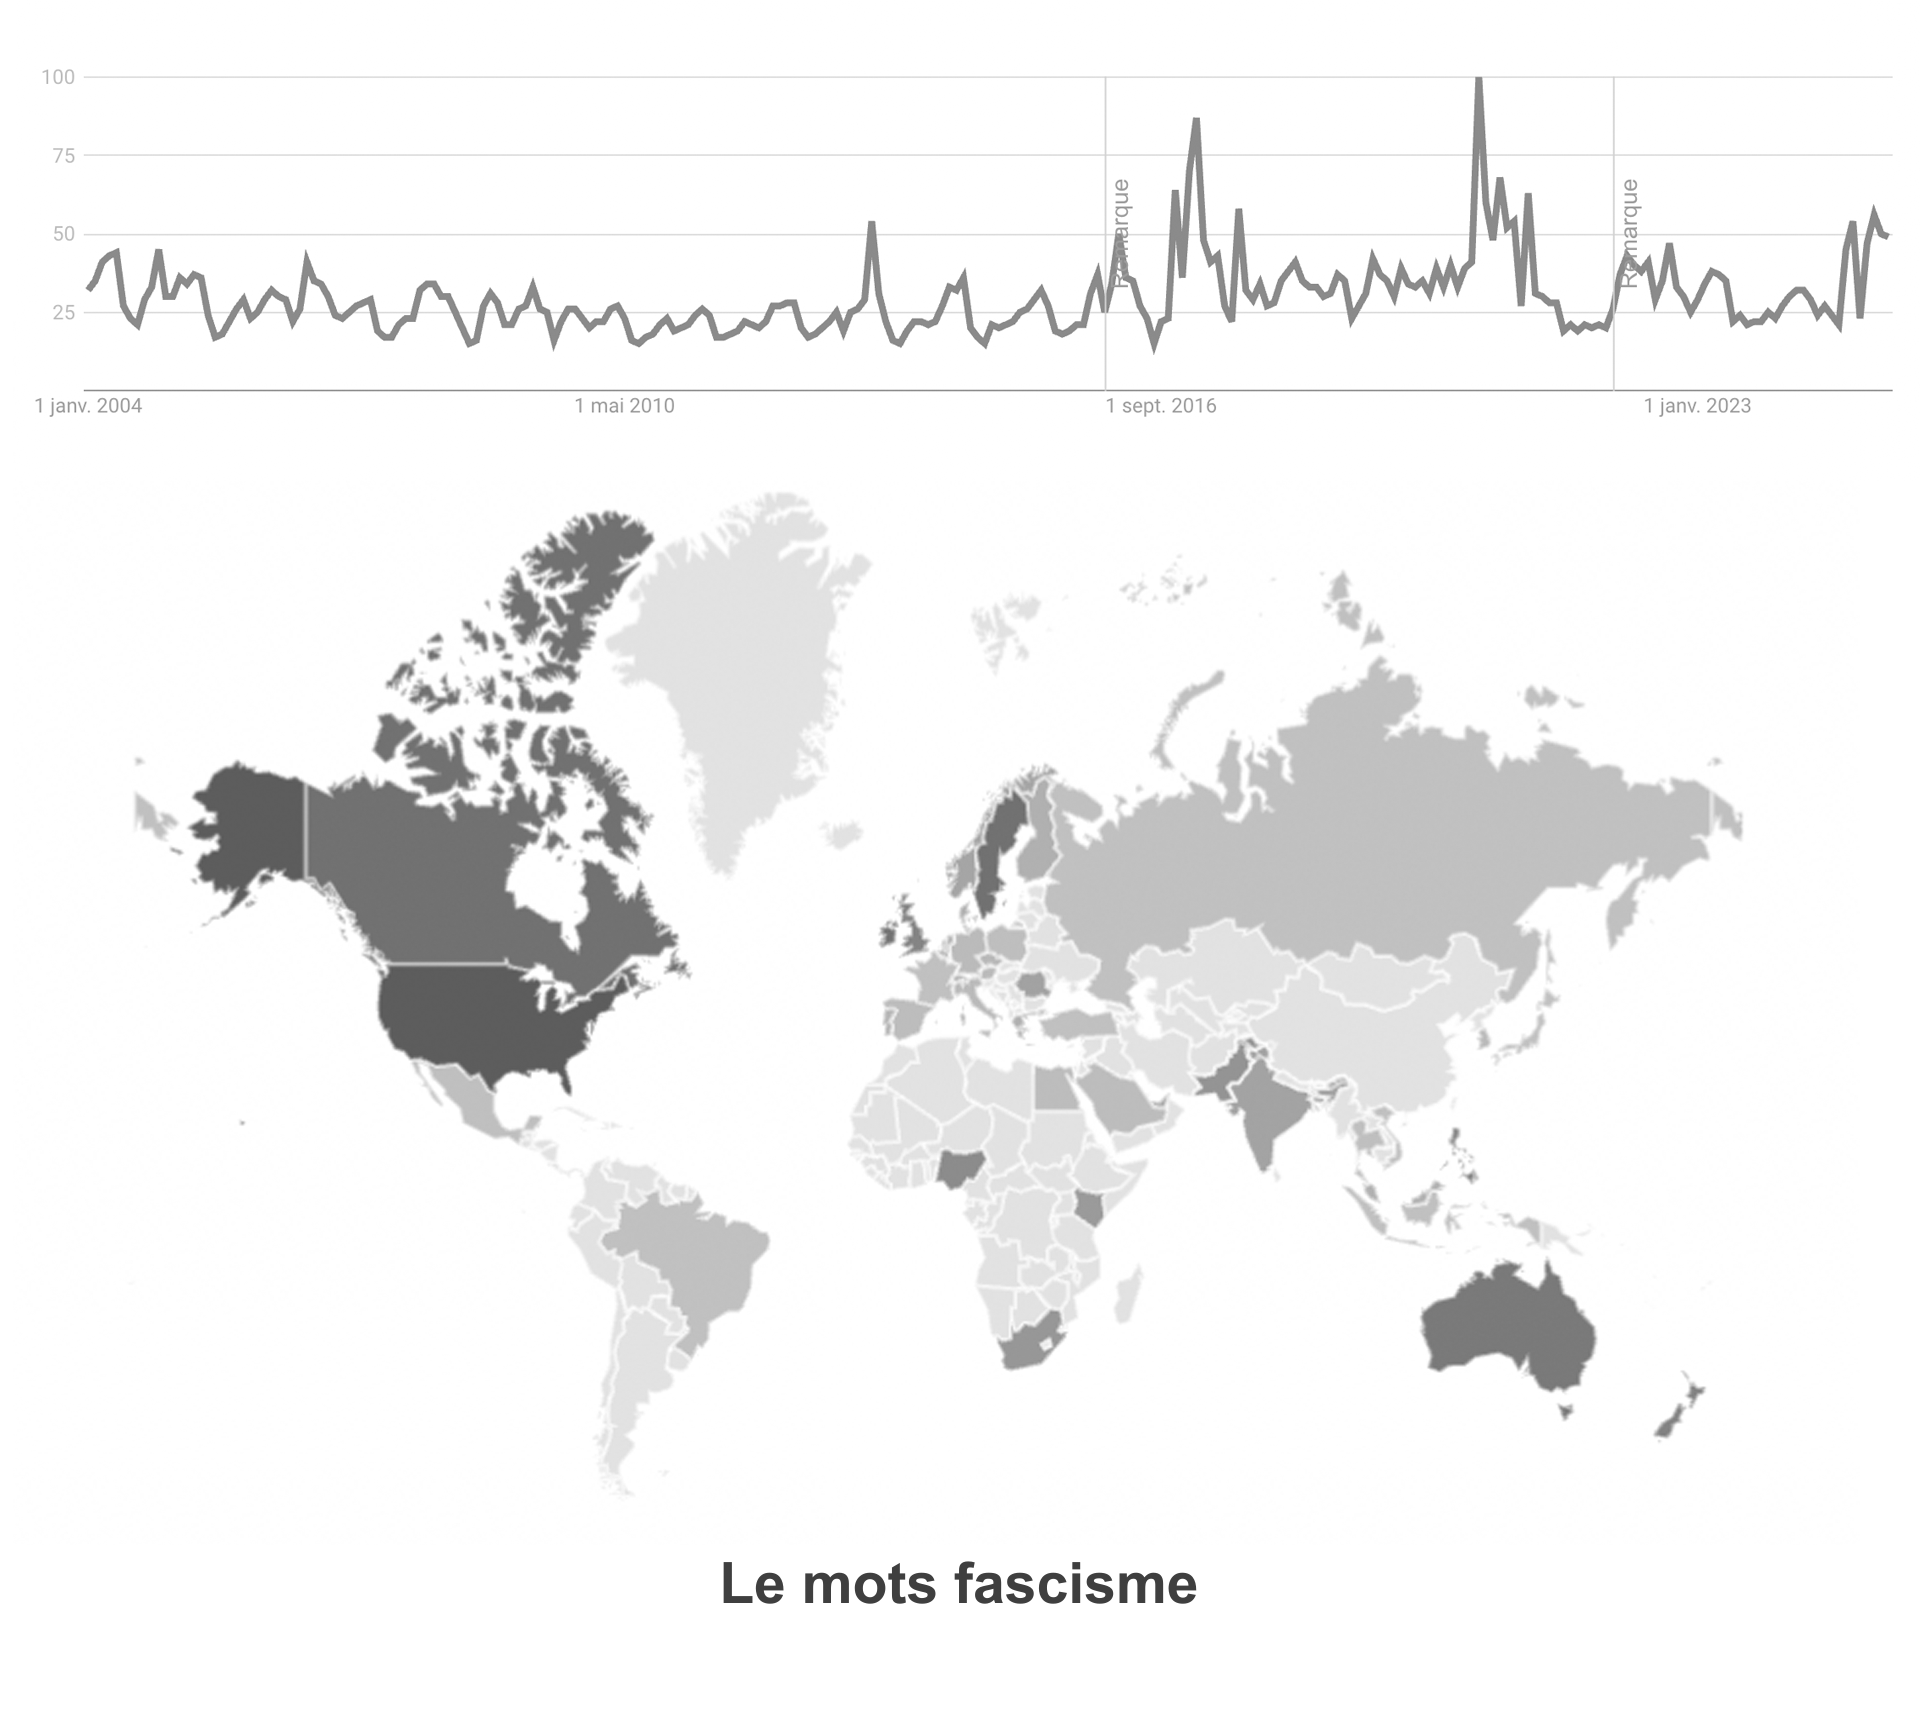
\includegraphics[keepaspectratio]{_i/Stats-Google.png}}

Depuis 2004, les requêtes Google avec le mot «fascisme» sont plus
fréquentes aux États-Unis que partout ailleurs, ce qui n’est peut-être
pas fortuit. La fréquence de ces requêtes ne fait que légèrement bondir
fin 2024, quand le duo Donald Trump/Elon Musk est aux portes de la
Maison-Blanche, comme si nous étions peu nombreux à nous inquiéter (en
tout cas, bien moins que ceux qui s’intéressent au fooball ou à la mode,
ce qui en soit est préoccupant).

Une question se pose: cette alliance entre politique et business
est-elle la réminiscence des alliances passées, un concours de
circonstances ou une tendance forte installée pour durer? Dans une
société de plus en plus technologique, la chose est-elle une fatalité?

Une observation à la fois historique et logique s’impose: quand la
centralisation s’accroît, les risques de totalitarisme augmentent car le
pouvoir se retrouve aux mains d’une élite qui se croit souvent capable
de régler les problèmes de tous.

Le sociologue Alain Bihr explique que le fascisme s’accompagne «d’une
concentration (un renforcement) et d’une centralisation (en termes
d’organisation interne) accrues du pouvoir politique au sein des
appareils d’État, au détriment des périphéries étatiques (les pouvoirs
publics locaux) et des organes de la société civile\footnote{Alain Bihr,
  ``Le fascisme ne passera plus'',
  \href{https://revue-refractions.net/fr}{\emph{Réfractions} n°\,34}.}.»
Autrement dit: le centre se renforce pendant que la périphérie se
délite.

Il se trouve que depuis le début du XXI\textsuperscript{e} siècle, nous
avons développé des technologies qui facilitent la concentration des
pouvoirs. Plus de centralisation donne plus de puissance à quelques-uns,
et ils centralisent davantage pour maximiser encore leurs pouvoirs, au
point de se griser d’eux-mêmes et devenir dangereux pour nous tous. Les
conditions sont réunies pour l’émergence de régimes autoritaires
renforcés par la technologie.

Dans \emph{The Atlantic} en février 2025, on peut lire\footnote{``DOGE
  Has ‘God Mode’ Access to Government Data'', \emph{The Atlantic}, 19
  février 2025, cité par Hubert Guillaud,
  \href{https://danslesalgorithmes.net/2025/03/04/doge-lefficacite-vraiment}{\emph{Dans
  les Algorithmes}}.}: «Aucune bonne raison ou argument ne peut être
avancé pour qu’une personne [Musk] ou une entité [le Doge, département
de l’efficacité gouvernementale dirigé par Musk] aient un tel accès à
autant d’agences gouvernementales contenant autant d’informations
sensibles. Même dans un seul bureau gouvernemental, l’accès
administratif complet à tous les systèmes est un privilège qui n’existe
pas. À l’échelle de l’ensemble du gouvernement, ce serait
incompréhensible.»

Comment en sommes-nous arrivés à inventer la centralisation ultime qui
pourrait préfigurer une de ces choses extrêmes imaginées par les auteurs
de science-fiction?

\section{\texorpdfstring{Aux racines de la
centralisation}{    }}\label{aux-racines-de-la-centralisation}

\textbf{~1960}. Dès leur naissance, les réseaux ancêtres d’internet sont
centralisés: un serveur dialogue avec chacun des ordinateurs connectés.
Pour communiquer entre eux, ces ordinateurs «client» contactent le
serveur, qui renvoie les messages vers les destinataires. Le serveur est
le centre du réseau, qualifié de réseau en étoile. Qui contrôle le
serveur contrôle le réseau. Aucune communication transversale entre
clients n’est possible.

\pandocbounded{\includegraphics[keepaspectratio]{_i/RéseauEtoile.png}}

\textbf{~1980}. Peu à peu les serveurs communiquent entre eux selon le
protocole Unicast\footnote{Sur l’Unicast, voir
  \href{https://fr.wikipedia.org/wiki/Unicast}{Wikipédia}.}: chaque
machine sur le réseau, client ou serveur, dispose d’une adresse IP
unique du type\,172.217.20.206 (Google) ou 31.13.71.36
(Facebook)\footnote{Les adresses IP changent fréquemment, contrairement
  aux noms de domaine qui pointent vers elles.}. N’importe quelle
machine peut communiquer avec n’importe quelle autre, mais les messages
doivent remonter de serveur en serveur, puis redescendre jusqu’aux
destinataires. Qui contrôle les serveurs contrôle le réseau.

\pandocbounded{\includegraphics[keepaspectratio]{_i/RéseauDistributed.png}}

Quand un client demande des données à un serveur, elles sont envoyées de
serveur en serveur jusqu’au client. Si un autre client demande les mêmes
données, elles sont renvoyées et ainsi de suite. Il existe souvent des
serveurs intermédiaires, appelés caches, qui évitent à la requête de
remonter jusqu’au serveur central pour être satisfaite, mais ce serveur
les contrôle. Quand le serveur censure des données, elles disparaissent
du réseau. Chaque serveur est un centre de pouvoir.

Par analogie, c’est comme si une lettre envoyée à votre voisin devait
remonter jusqu’à Paris avant de revenir à quelques mètres de chez vous.

Serveurs centralisés ne signifie pas que les données suivent toujours le
même chemin entre les serveurs. Le réseau est distribué pour qu’elles
atteignent leur cible, même si une partie du réseau tombe en panne.
Toujours par analogie, avant d’atteindre Paris, votre lettre peut passer
par Lyon, Toulouse ou Marseille, avant de revenir en passant par
Bordeaux, Nantes ou Strasbourg.

\textbf{~1985}. Pour faciliter l’identification des machines, on met en
place les serveurs DNS (Domain Name System) qui associent des noms de
domaine aux adresses IP. Saisir «google.com» dans notre navigateur web
revient à taper «172.217.20.206». C’est plus pratique, mais les serveurs
DNS, bien que distribués à la surface de la planète, restent
hiérarchisés et dépendent des serveurs centraux qui les contrôlent,
gérés par l’ICANN (Internet Corporation for Assigned Names and Numbers),
une organisation à but non lucratif de droit privé basée à Los Angeles.
Qui contrôle les DNS contrôle les noms d’accès sur le réseau.

\textbf{~1990}. Sur ce réseau, Tim Berners-Lee invente le web, une
surcouche qui simule une décentralisation totale. Les pages web pointent
les unes vers les autres, sans base de données centralisée des
liens\footnote{Pas de serveur centralisé pour les liens, mais ils
  utilisent les noms de domaine stockés dans les serveurs DNS.}. Tout le
monde se met à créer des contenus et à les relier. En quelques années,
le nombre de sites web explose, avec l’apparition des sites personnels.
Les lecteurs sautent de site en site, ils surfent, cliquant sur les
liens dans les articles. Une forme de correspondance ouverte et
multimodale s’engage, une nouvelle république des livres se construit en
temps réel, à une vitesse inédite. Mais si, à l’échelle du web, personne
ne peut censurer quoi que ce soit, le réseau reste censurable, puisqu’il
est toujours Unicast. Qui contrôle les serveurs contrôle le web.

\textbf{~1995}. On invente des protocoles de type Multicast\footnote{Sur
  le Multicast, voir
  \href{https://fr.wikipedia.org/wiki/Multicast}{Wikipédia}.}, où les
informations s’écoulent de machine en machine, chacune devenant un
client et un serveur pour d’autres clients. Les communications
transversales sont enfin possibles: vous pouvez envoyer une lettre
directement à votre voisin.

\pandocbounded{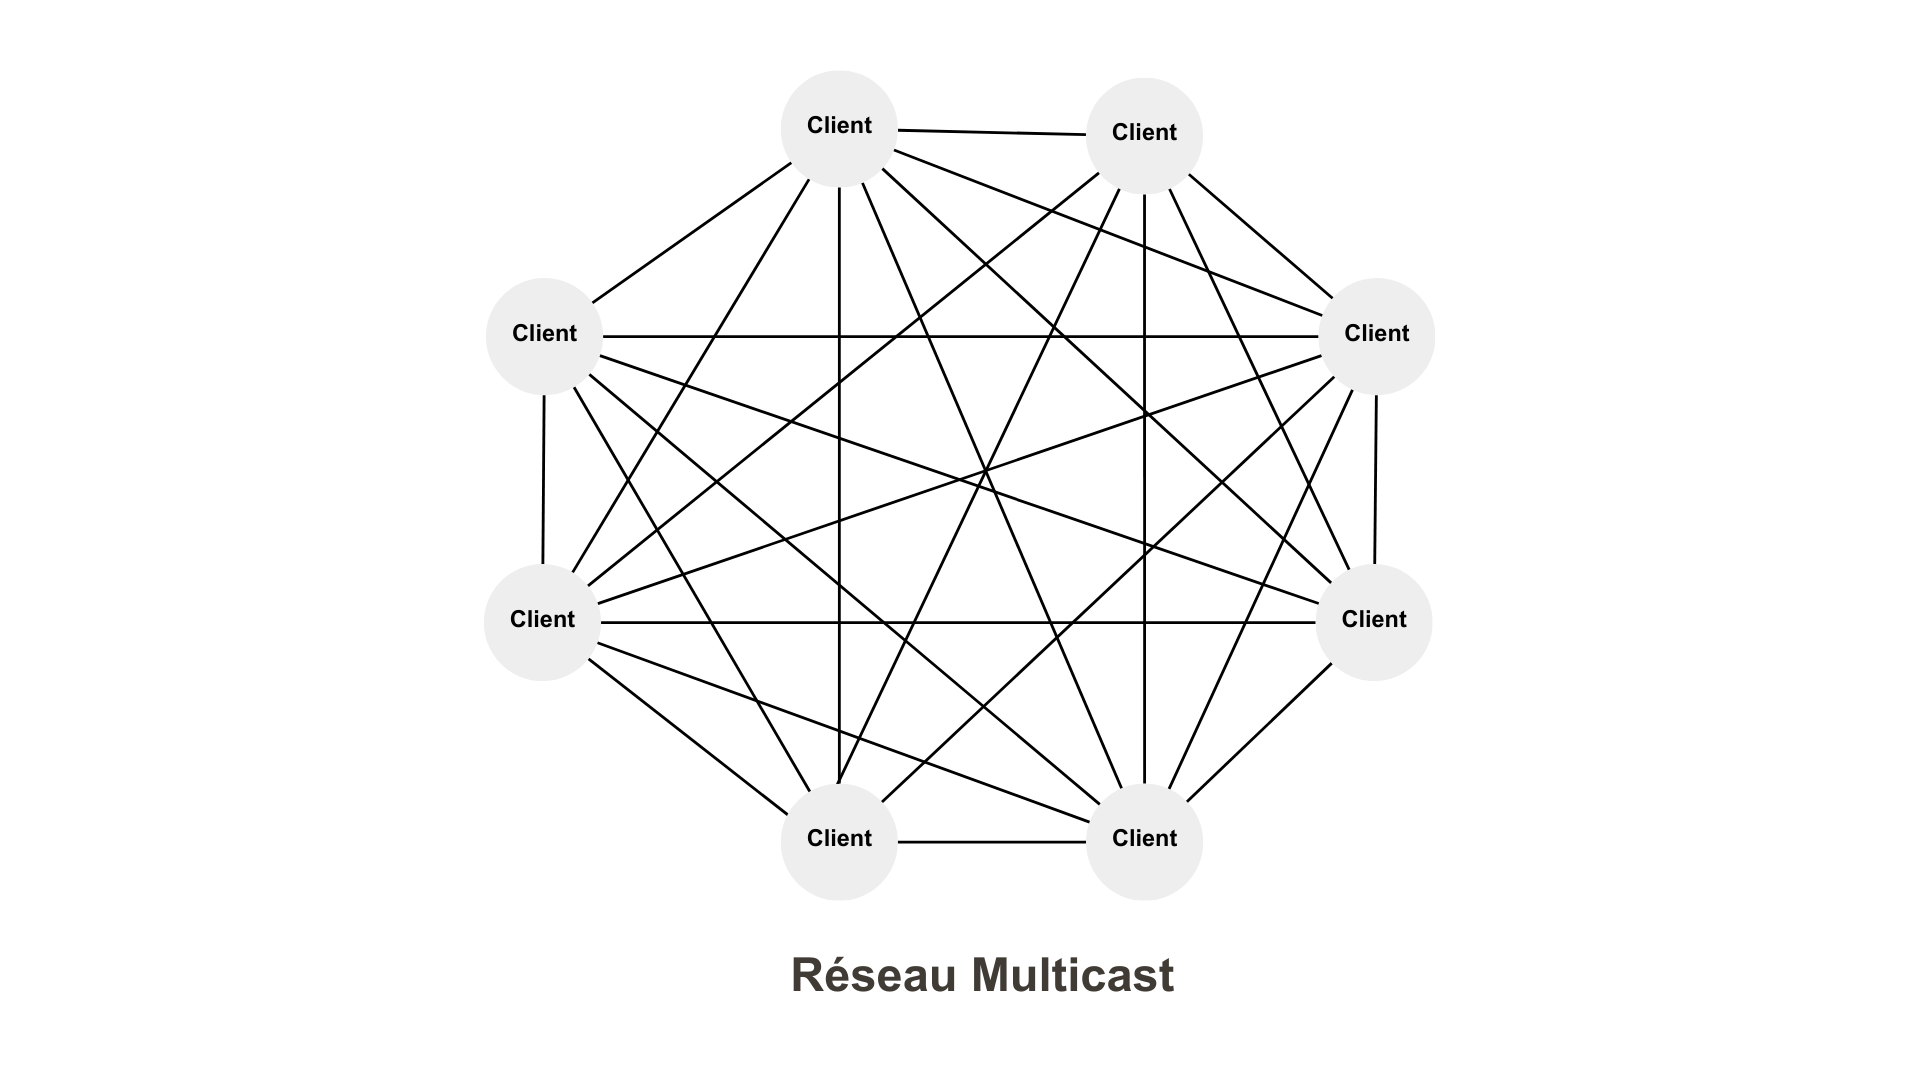
\includegraphics[keepaspectratio]{_i/Multicast.png}}

C’est la théorie. L’infrastructure Unicast est déjà si répandue que
personne n’envisage de la moderniser. Il aurait fallu remplacer tous les
routeurs, c’est-à-dire les moindres nœuds physiques du réseau pour leur
donner la capacité de transférer directement les messages aux
ordinateurs voisins plutôt que de les faire remonter vers les serveurs.

Au-delà du problème de coût, aucun industriel n’a intérêt au
développement du Multicast, puisqu’il implique de perdre le contrôle des
communications, même s’il est plus efficace énergétiquement: un fichier
transmis à un client peut être transféré à un autre sans que le serveur
initial intervienne.

Le Multicast, c’est comme acheter un livre, puis le prêter à un ami. Si
l’éditeur retire le livre de la vente, nous le possédons toujours et
pouvons continuer de le faire circuler.

\textbf{~2000}. Si le Multicast n’a jamais été déployé au niveau
matériel, il l’est en revanche sous forme de simulations logicielles,
généralement appelées P2P, pour communication de pair-à-pair. À la suite
d’Usenet (1979) et de Napster (1999), Gnutella est le premier protocole
totalement décentralisé dédié au partage de fichiers. Il devient
possible de communiquer transversalement sans supervision.

Une fois encore, c’est la théorie. Tout protocole de communication a une
signature. Les routeurs au niveau des fournisseurs d’accès peuvent
identifier les échanges, les bloquer ou les traquer. Selon les pays, au
nom de la défense des droits d’auteur, des programmes plus ou moins
invasifs de surveillance des usagers se mettent en place, notamment en
France avec Hadopi, mais ces programmes sont souvent inefficaces car de
nouvelles solutions techniques apparaissent, utilisant la cryptographie
et les VPN (Virtual Private Network). Le provider peut juste dire que
quelque chose de louche circule sur la ligne. Il doit choisir entre
laisser faire ou couper les échanges.

Parce que le P2P implique des échanges privés, sans supervision, son
usage n’est encouragé, ni par les gouvernements ni par les industriels
qui entendent garder le contrôle du réseau. Pour soutenir le
développement de l’Unicast, ils créent d’immenses salles des machines,
puis des datacenters.

\textbf{~2004}. Tim O’Reilly popularise la notion de
Web\,2.0\footnote{Tim O’Reilly, ``What Is Web 2.0?'', 30 septembre 2005,
  \href{https://www.oreilly.com/pub/a//web2/archive/what-is-web-20.html}{Oreilly}.}.
Il entérine une évolution en marche depuis le début des années\,2000: de
spectateurs nous devenons acteurs. Les plateformes de blogs facilitent
la publication. Nous nous faisons connaître par nos commentaires et nous
créons collectivement la blogosphère, un réseau social décentralisé
d’une remarquable efficacité organisé autour des auteurs et de leurs
écrits. En plus des liens dans les textes et les commentaires, les
listes de blogs amis affichées sur toutes les pages nous aident à
naviguer de blog en blog. C’est un âge d’or pour la liberté
d’expression.

\textbf{~2007}. Google s’affirme si incontournable que nous ne passons
presque plus que par lui pour trouver une information (60\,\% du marché
des moteurs de recherche, bientôt 80\,\%). Alors qu’avant on surfait, on
se met à googler. On fait de Google le maître du web. Sa régie
publicitaire AdSence génère des milliards de dollars de revenus. Le
principe: un algorithme glisse des liens publicitaires dans les
résultats de recherche, mais aussi dans tous les sites partenaires.

Google se met alors à lutter contre les liens artificiels, supposés
créés uniquement pour influencer son algorithme et faire monter certains
sites dans les résultats de recherche. Paradoxalement, les listes des
sites amis sur les blogs deviennent suspectes. Pour Google, elles n’ont
aucune raison éditoriale puisqu’elles n’étayent pas les articles (oublié
qu’elles constituent l’infrastructure de la blogosphère). Elles sont
considérées comme des publicités cachées, ou des tentatives de
manipulation de l’algorithme, donc pénalisées.

Il en va de même des liens dans les commentaires soudain pris comme des
tentatives de spammer l’algorithme, et même des liens trop nombreux dans
les articles. Cette politique répressive de Google se durcit peu à peu.
Pour rester présents dans les résultats de recherche, les blogs
suppriment les listes de sites amis, interdisent les liens dans les
commentaires, limitent le nombre de liens dans leurs articles et
finissent par détruire ce qui faisait l’essence de la blogosphère.
L’écosystème des sites interconnectés à la main commence à s’effondrer
et les algorithmes de Google décident de nos lectures\footnote{Dès,
  février 2004, lors de la mise à jour Brandy de l’algorithme Google, on
  découvre que la lutte s’intensifie contre les liens dits de peu de
  qualité. Cette politique ne cesse de se durcir au fil des années pour
  culminer en 2012 avec la version Penguin. Explications détaillées sur
  \href{https://www.impressiondigital.com/blog/key-google-algorithm-changes}{Impressiondigital.com}.}.

Ce n’est jamais ouvertement reconnu, mais tous ces liens jugés
artificiels par Google court-circuitent les fonctions de recherche, donc
court-circuitent Google, ce qu’il ne peut accepter: moins de liens,
c’est davantage de recherches, donc davantage de revenus\footnote{Laurent
  Lucas, ``Google Confirme Enfin que les Liens Externes ou Backlinks ne
  Sont pas Aussi Importants'', 2024. La véritable raison de la guerre
  contre les liens devient évidente: lutter contre le surf.}. Google
s’attaque au surf lui-même, cette possibilité de naviguer de site en
site.

Pour ma part, depuis 1998, j’éditais bonweb.com, un annuaire des
meilleurs sites web, version électronique de mon livre du même nom, qui
s’était hissé parmi les gros sites français. En novembre 2007, Google
nous a blacklistés, au prétexte que nous étions une ferme à liens, alors
que nos liens étaient choisis, éditorialisés, exactement comme dans un
\emph{Gault\&Millau} ou un \emph{Guide Michelin}\footnote{Thierry
  Crouzet, ``Google hégémonique'', 19 novembre 2007,
  \href{https://tcrouzet.com/2007/11/19/google-hegemonique/}{Tcrouzet.com}.}.
Décision unilatérale. Le trafic s’est aussitôt effondré. Qui contrôle
les serveurs et les algorithmes contrôle le Web et y impose sa
dictature. On bascule d’un web social à un web algorithmique.

\textbf{~2010}. Plus Google casse la blogosphère, plus il pousse les
internautes vers les réseaux sociaux naissants où ils retrouvent matière
à débat et lieux d’expression. Au début, aucun algorithme ne pilote les
conversations. Quand on a cent amis, ils voient tous nos messages et
réciproquement.

En parallèle, plus le trafic passe par Google, plus le référencement
pour apparaître en tête des résultats de recherche coûte cher, et mieux
s’en tirent les sites puissants, notamment les plateformes de vente à
distance et les réseaux sociaux. Des blogs survivent, mais isolés.

À mon échelle artisanale, je ne peux plus me faire entendre, sinon dans
ma communauté de fidèles. Durant l’âge d’or, les moteurs comme Google
généraient 50\,\% de mon trafic, sans que je fasse quoi que ce soit,
soudain presque plus rien, ou uniquement sur des articles anciens aux
titres provocateurs. Je perds mes deux sources premières de sang neuf,
le surf et le référencement. Il devient quasi impossible d’être
découvert par hasard. Le web est devenu déterministe, c’est-à-dire
achetable.

Initialement décentralisé, le web a été recentré par Google autour des
réseaux sociaux et de quelques plateformes, leur conférant un pouvoir
démesuré. Alors débute le règne des GAFAM (Google, Apple, Facebook,
Amazon, Microsoft et consorts).

Leur but n’est plus de nous informer ou de nous faire réfléchir, mais de
nous exposer aux publicités. Leur ambition: nous retenir, comme jadis le
faisaient les TV, à ceci près que nous produisons souvent nos propres
contenus (nos propres chaînes). Idée géniale! Les réseaux sociaux
tentent d’oblitérer l’internet extérieur à eux-mêmes. La technique est
simple: «Si tu postes des liens vers l’extérieur, tu seras moins vu.»
Même logique de pénalisation de la concurrence que celle de Google. Une
grande stratégie d’enfermement des audiences se déploie, doublée de
l’exploitation de nos données personnelles, allant de ce que nous
publions volontairement à tout ce que nous révélons par nos
comportements numériques.

Braudel et d’autres historiens ont montré que le capitalisme s’efforce
d’approprier des ressources gratuites ou quasi gratuites\footnote{Fernand
  Braudel, \emph{Civilisation matérielle, économie et capitalisme}; Karl
  Polanyi, \emph{La Grande Transformation}; Immanuel Wallerstein,
  \emph{Théorie du système-monde}.}. Après avoir exploité les esclaves,
puis les minerais, le capitalisme exploite nos données personnelles. On
entre dans la société dystopique de \emph{1984} anticipée par Orwell:
«Tout citoyen, ou du moins tout citoyen assez important pour qu’on le
surveille, pouvait être placé vingt-quatre heures sur vingt-quatre sous
le regard de la police et à portée de voix de la propagande officielle.»
On a basculé du capitalisme industriel au capitalisme cognitif ou de la
surveillance\footnote{Carlo Vercellone, ``Sommes-nous sortis du
  capitalisme industriel?'', 2003. Sur le capitalisme de surveillance
  voir Shoshana Zuboff, 2014,
  \href{https://la-rem.eu/2019/07/capitalisme-de-surveillance/}{\emph{La
  revue européenne des médias}}.}.

Une anecdote. Alors que j’écris ce texte, mon fils aîné arrive en
Andorre avec son école pour une semaine de ski. Il m’envoie un SMS pour
me dire que son opérateur lui facture la connexion. Je cherche sur
Google pour vérifier. Une heure plus tard, sur Facebook, une publicité
me propose d’acheter une eSim adaptable à la région géographique. Voici
un exemple de surveillance. Durant plusieurs jours, on tentera de me
vendre cette eSim.

Qui contrôle les serveurs contrôle les algorithmes, donc l’acquisition
des données. Plus rien n’est fortuit. Avant la numérisation du monde,
quand les lecteurs cherchaient un livre, ils visitaient leur librairie,
parcouraient les rayons et tombaient souvent sur des textes éloignés de
leurs centres d’intérêt. Le fan de SF et de BD que j’étais a ainsi
découvert Hemingway, Faulkner et les polars de Manchette. Si j’étais
sous influence, c’était sous celle de mon libraire et de son algorithme
personnel. Quand je changeais de boutique, je changeais d’algorithme,
alors que désormais il est difficile de s’émanciper des algorithmes.

Nous finissons par avaler une montagne de contenus indésirables placés
sous nos yeux pour nous maintenir \emph{in situ} et consommer des
publicités. Ces contenus altèrent notre imaginaire, notre philosophie,
notre conception du monde, nos opinions politiques, d’autant qu’ils
proviennent prétendument de nos «amis» et que nous leur accordons plus
confiance qu’aux informations proposées par les journalistes. Un réseau
social algorithmique n’a rien de social: c’est une machine à nous
emprisonner.

Par exemple, Spotify n’a aucun intérêt à nous faire écouter un genre
musical obscur, difficile, que nous n’aimerons pas (comme Amazon n’a
aucun intérêt à nous pousser vers des livres déroutants). Les
algorithmes sont prudents: ils étendent nos champs culturel, politique
et technique sans prise de risque. Seul notre espace de consommation les
intéresse.

Au début du web, on surfait, ce qui revenait à explorer pas à pas le
territoire numérique et à trouver des réponses par nous-mêmes, puis on a
googlé, demandant à un algorithme de nous fournir la supposée meilleure
réponse possible, désormais on scrolle, faisant défiler sans fin de haut
en bas des statuts sociaux hypnotiques dont nous nous moquons le plus
souvent.

\textbf{~2025}. Nous entrons dans une nouvelle époque, nous faisons
confiance aux IA qui composent leurs propres réponses. Leur
développement exponentiel nécessite d’immenses datacenters et une
centralisation de plus en plus extrême. Les oligarques deviennent si
puissants qu’ils manipulent les politiques. Qui contrôle les serveurs
contrôle les IA et les récits qu’elles nous donnent du monde.

Quand j’ai demandé à DeepSeek, l’IA chinoise, de me parler du lien entre
le fascisme et l’industrie, elle m’a affiché une réponse argumentée,
puis l’a effacée pour la remplacer par «Sorry, that’s beyond my current
scope. Let’s talk about something else.»

\section{\texorpdfstring{La dictature
algorithmique}{  }}\label{la-dictature-algorithmique}

On pourrait m’accuser d’exagérer, de noircir le tableau. Voici une autre
anecdote. Le 24 janvier 2025, j’ai publié sur mon blog un article sur le
technofascisme et l’ai annoncé sur trois plateformes:

\begin{itemize}
\tightlist
\item
  Sur Facebook où j’avais près de 5\,000 «amis», j’ai reçu 19 likes et 4
  partages\,(rendement 0,5\,\%).
\item
  Sur Bluesky où j’avais à peine plus de 200 «amis», j’ai reçu 9 likes
  et 4 partages (rendement 6,5\,\%).
\item
  Sur Mastodon où j’avais un peu plus de 600 «amis», j’ai reçu 80 likes
  et 90 partages (rendement 28\,\%).
\end{itemize}

Pas difficile de comprendre que quelque chose cloche sur Facebook. Mes
«amis» ne m’appartiennent plus. Ils ne sont pas mon audience, mais celle
de Facebook. Mon article n’y a été vu que par des proches intéressés par
le sujet traité. Dans le même temps, j’ai publié un texte plus
consensuel sur le vélo qui a été abondamment partagé et commenté.
Facebook est un réseau social à géométrie variable.

Si j’y avais publié mon article sur le vélo en intégralité plutôt que sa
simple annonce, il aurait été davantage lu: les lecteurs seraient restés
au contact de Facebook et de sa machine à clics.

Le rendement de mon article sur Mastodon s’explique parce que les
usagers de Mastodon sont particulièrement inquiets des extrémismes. Mais
cet effet communautaire ne justifie pas à lui seul l’écart dans le
nombre de réactions. Sur Facebook: un algorithme a pris en otage mon
audience. Il exploite la communauté que j’ai construite au fil des
années à ses propres fins. Voilà où nous en sommes sur un espace
initialement considéré comme le paradis de la libre expression. On est
libre de s’exprimer, mais pas de se faire entendre.

En amont des élections législatives allemandes du 23 février 2025, l’ONG
Global Witness a découvert que 64\,\% des contenus politiques
recommandés par l’algorithme de X et 78\,\% de ceux de TikTok sont liés
à l’extrême droite\footnote{\href{https://globalwitness.org/en/campaigns/digital-threats/tiktok-and-x-recommend-pro-afd-content-to-non-partisan-users-ahead-of-the-german-elections/}{globalwitness.org},
  ``TikTok and X recommend pro-AfD content to non-partisan users ahead
  of the German elections'', 21 février 2025.}. Preuve supplémentaire
des biais algorithmiques. Les points de vue polarisants et radicaux sont
favorisés car ils facilitent la viralité, provoquent davantage de clics
et de réactions, et donc s’entretiennent eux-mêmes\footnote{\href{https://www.pnas.org/doi/10.1073/pnas.1804840115}{Christopher
  A. Bail}, ``Exposure to opposing views on social media can increase
  political polarization'', \emph{PNAS}, 28 août 2018.}. Les algorithmes
ne sont pas nécessairement politisés mais, comme ils cherchent à
maximiser l’audience, ils sont prêts aux pires vilenies, ce qui en fait
des armes redoutables pour mettre en avant les thèses politiques les
plus contestables.

«Les réseaux sociaux récompensent l’outrance parce qu’elle suscite plus
d’engagement; cela revient à exploiter une faiblesse humaine», déclare
Bill Gates\footnote{David Remnick, ``Bill Gates: « Avec les réseaux
  sociaux et l’intelligence artificielle, je me rends compte que j’ai
  été assez naïf»'', 12 avril 2025,
  \href{https://www.vanityfair.fr/article/bill-gates-avec-les-reseaux-sociaux-et-intelligence-artificielle-je-me-rends-compte-que-jai-ete-assez-nai}{\emph{Vanityfair}}.}.

\section{\texorpdfstring{Une responsabilité
collective}{  }}\label{une-responsabilituxe9-collective}

Nous ne pouvons que nous reprocher cette trajectoire qui donne un
pouvoir incommensurable aux algorithmes et à leurs administrateurs, sans
contre-pouvoirs, hormis réglementaires, réglementations qui n’auront de
cesse d’être combattues, mise à sac commencée aux États-Unis sous
l’égide de Musk.

Nous sommes responsables d’avoir délaissé les sites d’informations
libres et indépendants, d’avoir renoncé au pluralisme, quitté les blogs.
Plutôt que de fouiller les recoins du web comme des librairies et des
disquaires, nous nous retrouvons dans les espaces censés nous offrir une
audience maximale. Pour nous séduire, les opérateurs vantent quelques
success-stories, tel ou tel influenceur qui gagne des millions, omettant
de préciser que nous ne parlons, le plus souvent, qu’à nos proches,
voire dans le vide.

Nous ressemblons à des insectes attirés par la lumière. Nous voulons
tous être là où elle brille et donnons ainsi du pouvoir à ceux qui se
transforment en soleil, au risque de perdre la tête et toute forme de
sagesse et de retenue. Il y a danger.

Cette brève histoire d’internet montre le lien entre une structure
technique, l’Unicast, et nos comportements grégaires, l’un et l’autre
s’entretenant comme l’œuf et l’huile dans la mayonnaise. «J’ai été
naïf», reconnaît Bill Gates. Nous avons tous été naïfs, et nous le
sommes toujours.

Qui contrôle les serveurs contrôle jusqu’à notre temps, et peut-être nos
rêves. Avant, nous étions sous l’influence d’un disquaire, d’un
libraire, d’un copain ou d’une copine, et chacun se construisait
indépendamment des autres. Nous cultivions notre idiosyncrasie, notre
unicité irréductible. Désormais, nous sommes sous l’influence de
quelques algorithmes. Les IA, elles-mêmes nourries de tous les savoirs,
moyennent, privilégient les opinions communes, et donc une fois de plus
normalisent tout en appliquant les biais glissés par leurs développeurs,
en toute opacité, mais toujours avec le désir de nous maintenir \emph{in
situ}, donc avec le risque de pousser des idées nauséeuses.

Note\,3 d’Evgueni Zamiatine: «Chaque matin, avec une précision
sextuplée, à la même heure et à la même minute, par millions, nous nous
levons comme si nous ne faisions qu’un. À la même heure, par millions,
nous nous mettons Unitairement au travail, et le soir, Unitairement,
nous terminons notre journée.» Dans la note\,8: «Nous sommes la moyenne
arithmétique la plus heureuse… Comment est-ce que vous dites?
L’intégration du zéro à l’infini –\,du crétin jusqu’à Shakespeare…»

\section{\texorpdfstring{Le piège du
technosolutionnisme}{   }}\label{le-piuxe8ge-du-technosolutionnisme}

Les technocapitalistes derrière les algorithmes orchestrent une
uniformisation d’un genre nouveau. Leur stratégie est imparable: nous
donner l’illusion de la liberté, nous persuader que nous pouvons tout
dire jusqu’à oublier nos chaînes. C’est une dictature douce, subversive,
invisible, insidieuse.

Si un type de contenu nous éloigne de la plateforme, il nous sera
présenté moins souvent, et inversement. Il se produit alors un
renforcement de ce qui est plébiscité —les spécialistes parlent
d’homophilie. Si vous prêtez attention à un article antivax, on vous en
proposera d’autres jusqu’à ce que vous deveniez vous-même antivax. Vous
commencerez à liker, puis à partager, puis à être le vecteur d’une
idéologie dont vous n’étiez au départ que simple curieux. Vous serez
d’autant plus enthousiaste que vous recevrez beaucoup de likes.

Les technocapitalistes se moquent souvent de «la vérité» ou de ce qui
est bon pour nous —par exemple, TikTok encourage l’anorexie\footnote{Antoine
  Blanchet, ``Tentative de suicide, anorexie… Sa fille a vécu un
  calvaire : TikTok a agi comme une drogue'', 20 novembre 2024,
  \href{https://actu.fr/ile-de-france/creteil_94028/tentative-de-suicide-anorexie-sa-fille-a-vecu-un-calvaire-tiktok-a-agi-comme-une-drogue_61883195.html}{Actu.fr}.}.
Ils n’ont qu’une visée utilitariste: nous maintenir chez eux, quitte à
nous bourrer le cerveau d’absurdités, voire d’idées dangereuses. Voilà
pourquoi ils militent pour la liberté d’expression totale: ils ont
compris qu’il y a toujours des gens pour aimer les pires théories, donc
pour rester les consommer. La liberté d’expression totale revient à
maximiser le nombre de filets jetés à la mer pour pêcher des poissons,
vous, nous, moi. Leurs mailles sont si entremêlées qu’il devient
difficile de résister.

Orwell dans \emph{1984}: «L’histoire n’est plus qu’un palimpseste,
soigneusement effacé et récrit aussi souvent que nécessaire. Une fois la
rectification effectuée, il devient impossible de prouver qu’il y a eu
falsification.» Il ajoute: «Qui contrôle le passé contrôle l’avenir, qui
contrôle le présent contrôle le passé.»

Dans les dictatures, la voix du Parti unique s’impose à tous. Sur les
plateformes centralisées supervisées par les algorithmes s’impose la
voix la mieux capable de nous emprisonner dans son filet, peu importe sa
couleur politique. Vu de très haut, un réseau social semble obéir au
pluralisme le plus extrême, mais, en zoomant, on constate que chacun
d’entre nous n’est exposé qu’à un nombre restreint de perspectives. À
notre échelle, le pluralisme global se transforme en monologue. Nous
aboutissons au monisme caractéristique des dictatures.

Loin d’être dupe, le technocapitaliste jouit de son pouvoir sur les
masses. Plus ses outils d’emprisonnement progressent, plus il se croit
tout-puissant et se persuade que la technologie peut régler même les
problèmes qu’elle a provoqués en premier lieu.

Cette ferveur solutionniste, cette croyance en la possibilité de
solutions simples, qui seraient uniformément imposées à tous, est une
autre caractéristique du totalitarisme. Une fois la Terre invivable, il
nous suffira de partir sur Mars, donc inutile de se préoccuper du
réchauffement climatique. Ainsi, le technocapitaliste, bientôt adepte du
technosolutionnisme, finit souvent par devenir un danger collectif.
Enfiévré par ses grandes idées, par sa richesse et son pouvoir sur les
consciences, il néglige la diversité des particularités locales et
individuelles. Seule la fuite en avant l’intéresse, quitte à entraîner
le monde à sa perte.

\section{\texorpdfstring{La chose mise à
l’épreuve}{    }}\label{la-chose-mise-uxe0-luxe9preuve}

J’ai essayé de décrire la naissance de la chose, et d’expliquer ce qui
la rend possible, l’Unicast, couplé à notre grégarisme, parce qu’en
premier lieu, si nous nous moquions de ce que les autres pensent de
nous, nous ne passerions pas notre temps sur les réseaux sociaux.

Umberto Eco a établi une liste des quatorze points communs à tous les
fascismes\footnote{\href{https://www.lesnouveauxdissidents.org/single-post/2017/07/24/umberto-eco-14-signaux-pour-reconna\%C3\%AEtre-le-fascisme}{Umberto
  Eco}, ``Ur-Fascisme'', 1995.}. Assistons-nous à l’avènement d’un
nouveau fascisme ou faut-il adopter une autre dénomination?

1/\,«\emph{La première caractéristique du fascisme éternel est le culte
de la tradition. Il ne peut y avoir de progrès dans la connaissance. La
vérité a été posée une fois pour toutes, et on se limite à interpréter
toujours plus son message obscur.»}

Les technocapitalistes n’ont rien de passéistes puisqu’ils promeuvent
les nouvelles technologies, mais nombre d’entre eux soutiennent Trump et
son slogan MAGA (\emph{Make America Great Again}). C’est sur le plan des
valeurs qu’ils peuvent être passéistes, avec le fantasme d’une Amérique
idyllique qui aurait disparu, une Amérique masculiniste, une Amérique
conquérante.

L’Unicast symbolise également le passéisme à travers la centralisation,
le pouvoir du centre du système sur tous ses périphériques. L’Unicast
impose un système monarchiste, voire féodal. C’est un technoféodalisme
selon Yanis Varoufakis ou Cédric Durand\footnote{Yanis Varoufakis,
  \emph{Technofeudalism}, 2023. Cédric Durand, \emph{Techno-féodalisme},
  2020.}. Il veut faire de nous des serfs, des piles énergétiques comme
dans \emph{Matrix}.

La vérité? Il n’y a plus de vérité. On a basculé dans la post-vérité.
Celui qui reçoit le plus de likes a raison, point. Il peut se
contredire. C’est sans importance. Quand le monarchiste s’accrochait à
la nature divine du roi ou le fasciste à la supériorité de sa race, le
nouvel adepte de la chose ne s’attache à aucune vérité, seulement à ce
qui le sert sur le moment. C’est un nombriliste. On serait plutôt du
côté du technoégoïsme, du technocynisme ou du technomépris. Nous sommes
donc très loin du fascisme.

2/\,\emph{«Le conservatisme implique le rejet du modernisme. Le rejet du
monde moderne se dissimule sous un refus du mode de vie capitaliste,
mais il a principalement consisté en un rejet de l’esprit de 1789 (et de
1776, bien évidemment Déclaration d’indépendance des États-Unis). La
Renaissance, l’Âge de Raison sonnent le début de la dépravation
moderne.»}

Trump et ses soutiens s’opposent au wokisme, à l’homosexualité, à
l’avortement… autant de positions contre le «modernisme». Mais refus du
capitalisme, non, bien au contraire. Nous assistons à une exacerbation
du capitalisme, un capitalisme où tous les moyens sont bons, même le
mensonge, les fake news, la manipulation des opinions (ce qui revient à
renoncer à la raison et à l’esprit des Lumières). C’est même un
capitalisme contre l’idée d’indépendance puisqu’il aspire à soumettre
tous les acteurs à la loi du plus fort. C’est un capitalisme dépourvu
d’éthique qui n’obéit plus qu’à l’idéal de rentabilité. Cette perte de
sens éthique fait penser aux époques de décadence. Vivons-nous une
technodécadence? Sans doute, si nous continuons à suivre la route de
l’Unicast.

3/\,\emph{«Le fascisme éternel entretient le culte de l’action pour
l’action. Réfléchir est une forme d’émasculation. En conséquence, la
culture est suspecte en cela qu’elle est synonyme d’esprit critique. Les
penseurs officiels fascistes ont consacré beaucoup d’énergie à attaquer
la culture moderne et l’intelligentsia libérale coupables d’avoir trahi
ces valeurs traditionnelles.»}

Trump aime taper sur la table, balancer ses vérités, les imposer par la
force. Il refuse la discussion, l’argumentation, la théorisation. Il
s’entoure de technocapitalistes plutôt que d’intellectuels. Pour eux,
réussir, c’est entreprendre. On ne mesure plus la profondeur de la
pensée, mais l’épaisseur du compte en banque. Celui qui échoue est
fautif (comme si tout le monde pouvait réussir selon les critères du
capitalisme —ce qui est un non-sens puisque ce modèle exige
l’exploitation d’une majorité par une minorité). On est bien dans le
culte de l’action pour l’action (on agit souvent avant même de
réfléchir).

4/\,\emph{«Le fascisme éternel ne peut supporter une critique
analytique. L’esprit critique opère des distinctions, et c’est un signe
de modernité. Dans la culture moderne, c’est sur le désaccord que la
communauté scientifique fonde les progrès de la connaissance. Pour le
fascisme éternel, le désaccord est trahison.»}

Pour éviter la critique, Trump et ses supporteurs s’attaquent à la
science et aux scientifiques. De leur côté, les algorithmes ne musellent
pas les critiques: encore une fois, ils se moquent du fond et se
contentent de mesurer. Comme les critiques, surtout sérieuses et
argumentées, engendrent peu de clics, elles sont enterrées. La mécanique
algorithmique déployée s’oppose à l’esprit des Lumières.

5/\,\emph{«En outre, le désaccord est synonyme de diversité. Le fascisme
éternel se déploie et recherche le consensus en exploitant la peur innée
de la différence et en l’exacerbant. Le fascisme éternel est raciste par
définition.»}

Fermeture des frontières et renvoi des étrangers chez eux ne font que
traduire la prévalence de la xénophobie, c’est vrai pour Trump, aussi
pour Musk, mais pas pour tous les technocapitalistes, même si leurs
algorithmes favorisent l’homophilie et la radicalité, donnant plus de
poids aux discours xénophobes. Souvent cette xénophobie n’est pas
voulue, mais s’avère rentable. Quand le technocapitaliste tolère cette
rentabilité, il devient technohypocrite.

6/\,\emph{«Le fascisme éternel puise dans la frustration individuelle ou
sociale. C’est pourquoi l’un des critères les plus typiques du fascisme
historique a été la mobilisation d’une classe moyenne frustrée, une
classe souffrant de la crise économique ou d’un sentiment d’humiliation
politique, et effrayée par la pression qu’exerceraient des groupes
sociaux inférieurs.»}

Trump a promis aux classes moyennes de retrouver une prospérité
mythique. Une belle histoire à laquelle suffisamment d’Américains ont
cru pour l’élire président à deux reprises. Il s’est appuyé sur la peur
des lendemains, sur l’incertitude. Il a fait de la politique
paternaliste comme tous les fascistes en désignant comme ennemis les
étrangers ainsi que les bénéficiaires des prestations sociales.

Mais Trump est arrivé au pouvoir parce que les algorithmes ont favorisé
la propagation de son discours, non parce que les technocapitalistes y
adhéraient, mais parce qu’ils ont mis en place des outils le rendant
audible. Il s’agit encore une fois d’une complicité flagrante, même si
elle n’a rien d’idéologique. Elle se répétera partout où les algorithmes
ne seront pas soumis à des règles éthiques, par exemple des exigences de
véracité.

Quand la maximisation des revenus prime, on en arrive presque
nécessairement à valoriser les extrémismes dans notre monde Unicast. Le
technocapitaliste finit lui-même par devenir la victime des thèses qu’il
a contribué à amplifier, même si au départ il ne les prenait pas au
sérieux. Les manipulations ne sont pas planifiées, mais résultent d’un
processus d’amplification par effet de réseau. Ce que croit Trump n’est
pas ce que croient les technocapitalistes, mais ils le tolèrent, ce qui
fait d’eux des technocollabos.

7/\,\emph{«Aux personnes privées d’une identité sociale claire, le
fascisme éternel répond qu’elles ont pour seul privilège, plutôt commun,
d’être nées dans un même pays. C’est l’origine du nationalisme. En
outre, ceux qui vont absolument donner corps à l’identité de la nation
sont ses ennemis. Ainsi y a-t-il à l’origine de la psychologie du
fascisme éternel une obsession du complot, potentiellement
international. Et ses auteurs doivent être poursuivis. La meilleure
façon de contrer le complot est d’en appeler à la xénophobie. Mais le
complot doit pouvoir aussi venir de l’intérieur.»}

\emph{Make America Great Again} est le slogan d’un nationalisme
obsessionnel, faisant de tous les autres pays des adversaires. Trump et
Musk avec lui se font les propagateurs de nombreuses théories du
complot. Ils sont fascistes à ce titre, mais les autres
technocapitalistes pourraient du jour au lendemain adhérer à d’autres
théories si elles s’avéraient plus rentables.

Leur idéologie se résume à ce qui les arrange à un moment donné. Ils se
placent au-dessus de la société. Ils se moquent des dérèglements
climatiques parce qu’ils pensent ne jamais en subir les conséquences
(ils se trompent -\,un jour, des désespérés s’en prendront à eux).

8/\,\emph{«Les partisans du fascisme doivent se sentir humiliés par la
richesse ostentatoire et la puissance de leurs ennemis. Les
gouvernements fascistes se condamnent à perdre les guerres entreprises
car ils sont foncièrement incapables d’évaluer objectivement les forces
ennemies.»}

Un discours difficile à tenir par des ultrariches, mais ils le tiennent
néanmoins, surtout Trump, qui accuse les alliés d’hier d’avoir pillé
l’Amérique. Les technocollabos perdront-ils la guerre? Oui, parce que
toutes les guerres finissent par être perdues.

9/\,\emph{«Pour le fascisme éternel, il n’y a pas de lutte pour la vie
mais plutôt une vie vouée à la lutte. Le pacifisme est une compromission
avec l’ennemi et il est mauvais à partir du moment où la vie est un
combat permanent.»}

Trump comme Musk sont violents, toujours dans la confrontation. C’est
écraser pour ne pas être écrasé, mais rien d’original dans le monde
capitaliste.

10/\,\emph{«L’élitisme est un aspect caractéristique de toutes les
idéologies réactionnaires. Le fascisme éternel ne peut promouvoir qu’un
élitisme populaire. Chaque citoyen appartient au meilleur peuple du
monde; les membres du parti comptent parmi les meilleurs citoyens;
chaque citoyen peut ou doit devenir un membre du parti.»}

Trump ne cesse d’user de cette rhétorique, mais les technocapitalistes
ont une approche supranationale guère compatible avec ce credo.

11/\,\emph{«Dans une telle perspective, chacun est invité à devenir un
héros. Le héros du fascisme éternel rêve de mort héroïque, qui lui est
vendue comme l’ultime récompense d’une vie héroïque.»}

Un point qui sans doute ne vaut pas pour le technocapitaliste, à moins
qu’il ne s’agisse de risquer sa vie pour réussir dans le business:
l’entrepreneur comme héros, ce qui revient à piller tous les autres
corps sociaux (santé, éducation, humanitaire, culture…).

12/\,\emph{«Le fasciste éternel transporte sa volonté de puissance sur
le terrain sexuel. Il est machiste (ce qui implique à la fois le mépris
des femmes et l’intolérance et la condamnation des mœurs sexuelles hors
normes: chasteté comme homosexualité).»}

Trump et Musk comme parangons de cette attitude avec en parallèle des
algorithmes qui amplifient la sexualisation. Mais généraliser à tous les
technocapitalistes paraît difficile.

13/\,\emph{«Le fascisme éternel se fonde sur un populisme sélectif, ou
populisme qualitatif pourrait-on dire. Le Peuple est perçu comme une
qualité, une entité monolithique exprimant la Volonté Commune. Étant
donné que des êtres humains en grand nombre ne peuvent porter une
Volonté Commune, c’est le Chef qui peut alors se prétendre leur
interprète. Ayant perdu leurs pouvoirs délégataires, les citoyens
n’agissent pas; ils sont appelés à jouer le rôle du Peuple.»}

Populisme, oui, puisqu’il s’agit de ne retenir que ce qui plaît, mais la
Volonté Commune n’existe pas pour les algorithmes puisqu’ils cultivent
l’homophilie. Ils ne cherchent pas à imposer une théorie mais que chacun
s’enferme dans sa sienne.

Toutefois, à l’intérieur d’un groupe, l’algorithme a besoin de
porte-voix qui brillent pour attirer les insectes. À ce titre, Trump est
un influenceur politique, avec le risque que la démocratie soit
confisquée par les influenceurs, donc par les algorithmes, \emph{in
fine} par les technocollabos.

14/\,\emph{«Le fascisme éternel parle la Novlangue. La Novlangue,
inventée par Orwell dans} 1984, \emph{est la langue officielle de
l’Angsoc, ou socialisme anglais. Elle se caractérise par un vocabulaire
pauvre et une syntaxe rudimentaire de façon à limiter les instruments
d’une raison critique et d’une pensée complexe.»}

Les algorithmes ne poussent pas une langue simplifiée mais une multitude
de dialectes dans chacun des groupes. Ils n’uniformisent pas à l’échelle
globale, mais à l’échelle locale.

\section{\texorpdfstring{Comment nommer la
chose?}{   }}\label{comment-nommer-la-chose}

Nous n’assistons donc pas à l’avènement d’un fascisme stricto sensu.
Résumé des caractéristiques de cette chose:

\begin{itemize}
\tightlist
\item
  non idéologique (à part de faire de l’utilitarisme une idéologie),
\item
  centralisatrice,
\item
  élitiste,
\item
  méprisante,
\item
  non éthique,
\item
  mercantile,
\item
  nombriliste,
\item
  abêtissante,
\item
  illusionniste,
\item
  mensongère,
\item
  addictive,
\item
  enfermante,
\item
  populiste,
\item
  autoritariste.
\end{itemize}

J’ai utilisé des mots comme technocollabos (je ne vois pas comment
appeler autrement ceux qui jouent le jeu des algorithmes),
technoféodalistes (nouveaux aristocrates qui nous réduisent à l’état de
serfs consentants), technoégoïstes ou technocyniques (qui ne pensent
qu’à eux-mêmes). J’aurais pu parler de technoarrivistes, navigant à vue,
sans la moindre préoccupation des enjeux historiques. Tout cela conduit
à un populisme né des algorithmes rendus surpuissants par l’Unicast.

\pandocbounded{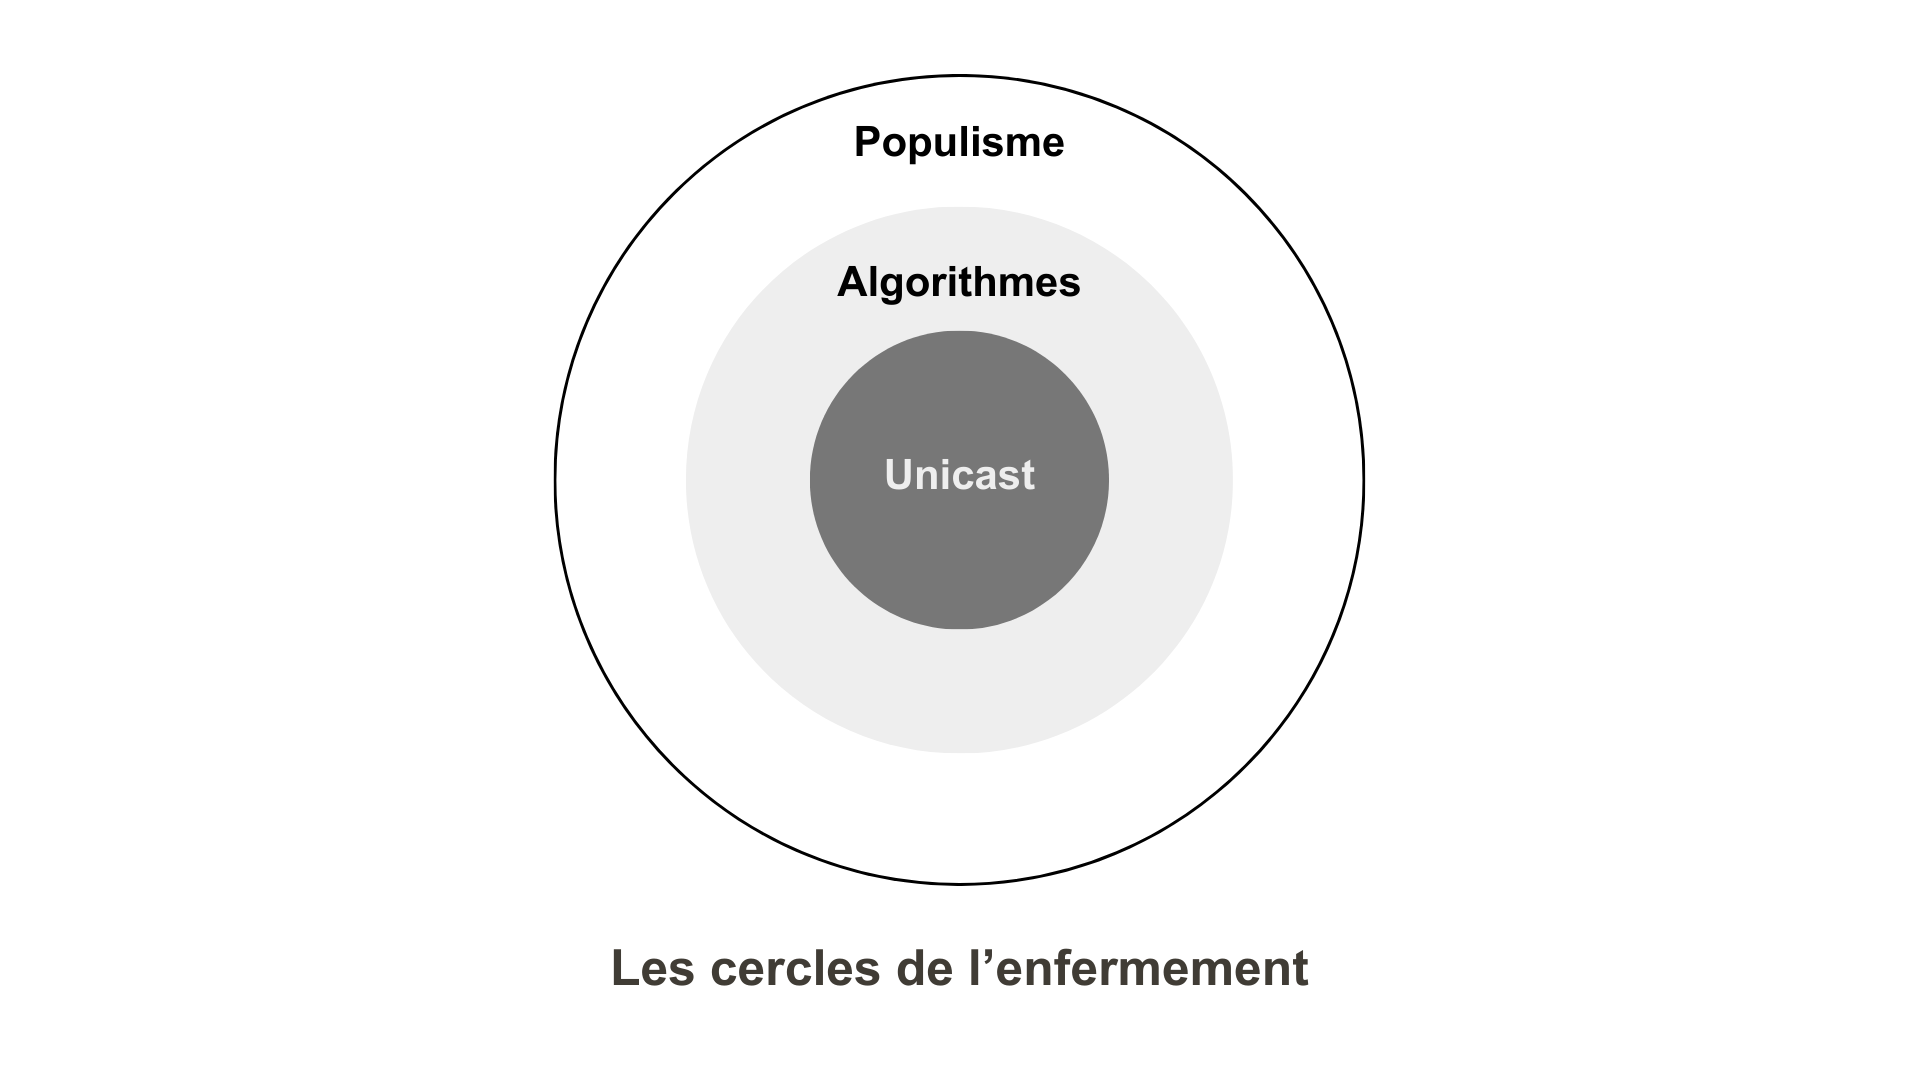
\includegraphics[keepaspectratio]{_i/TroisCouches.png}}

Je ne trouve toujours pas de nom pour la chose. J’ai pensé à Unicratie
pour désigner une forme d’influence globale à travers l’Unicast, avec
«cratie» qui vient du grec ancien kratos, signifiant «pouvoir», «force»
ou «autorité». Autrement dit le pouvoir de l’Unicast. On pourrait lui
opposer la Multicratie, c’est-à-dire le pouvoir du Multicast, un pouvoir
qui n’aurait rien de centralisé, qui serait distribué, coopératif,
bienveillant.

Ça reste trop technique. Pas susceptible d’incarner la chose, de nous
faire prendre conscience de sa malveillance. Je ne pense pas qu’il soit
nécessaire d’utiliser le préfixe «techno» ou «cyber», parce que le
problème n’est pas la technologie en général mais certaines technologies
numériques, celles qui renforcent des tendances et en atténuent d’autres
pour servir des intérêts centralisés, celles qui nous persuadent de
notre singularité tout en nous enfermant dans des bulles de réalités
hypothétiques. Il m’arrive de penser idiocratie, parce que la chose
tente de faire de nous des idiots pour mieux nous soumettre, mais en
rien des idiots ne créent les algorithmes. Il subsiste une volonté
derrière la chose, un consentement d’une élite, une acceptation des
masses.

C’est comme si nous tous ou presque renoncions à notre liberté: les
technocapitalistes de faire autrement, de gagner moins, nous autres de
renoncer à leurs outils. Un aveuglement généralisé nous conduit au pire,
comme avec les bouleversements climatiques. Nous savons et nous
continuons sans rien changer. La chose cultive notre masochisme.

Quand je pense à la chaîne de causalité: Unicast, Algorithmes,
Populisme, j’ai en tête UAP, sigle d’une assurance française. J’aurais
préféré un acronyme, mais les mots sont les mots, et UAP fait rire
plutôt que peur.

Peut-être est-il encore trop tôt pour nommer. Nous ne la comprenons pas
assez la chose pour la désigner, mais peut-être que la circonscrire
suffit à la combattre, car ce régime fou, presque inhumain, n’est pas
une fatalité.

\chapter{\texorpdfstring{Le livre: arme de
résistance}{    }}\label{le-livre-arme-de-ruxe9sistance}

Dix mai 1933, Munich. Des étudiants hitlériens escortent des camions
chargés de 20\,000\,livres jusqu’à la place de l’Opéra où ils les
brûlent. Parmi eux, les œuvres d’Heinrich Heine, Karl Marx, Sigmund
Freud, Albert Einstein, Franz Kafka, Stefan Zweig, Felix Mendelssohn.
Des auteurs juifs. Joseph Goebbels prononce un discours durant
l’autodafé.

En 1953, Ray Bradbury écrit dans \emph{Fahrenheit\,451}: «Un livre est
un fusil chargé dans la maison d’à côté. Brûlons-le. Déchargeons l’arme.
Battons en brèche l’esprit humain.»

Pourquoi les totalitaristes craignent-ils les livres? Réponse: il s’agit
d’une technologie Multicast difficile à contrôler.

Pourquoi Multicast? On peut comparer un éditeur à un serveur de
contenus. Il existe une myriade d’éditeurs, certains indépendants,
d’autres agrégés dans de grands groupes. Comme les serveurs, les
éditeurs contrôlent les contenus diffusés. Le plus souvent, ils ne les
envoient pas directement aux libraires, mais d’abord aux diffuseurs,
assimilables à des caches, où se servent les libraires qui choisissent
les titres à vendre (ils sont des clients). Ce réseau reste hiérarchisé,
donc contrôlable: si un éditeur cesse d’alimenter son diffuseur, les
libraires finissent par manquer de livres.

Dans la pratique, j’ai vu des librairies m’orienter vers des librairies
amies où trouver un livre épuisé. C’est un peu comme si, à travers les
lecteurs, les librairies communiquaient transversalement selon une
logique Multicast, échappant en partie au contrôle des distributeurs et
des éditeurs.

Après leurs achats, les lecteurs peuvent échanger leurs livres avec
d’autres lecteurs, encore une fois selon une logique Multicast. Les
bibliothèques publiques amplifient ces échanges, tout comme les boîtes à
livres. Plus il existe de lieux de vente et d’échange, mieux les livres
échappent au contrôle des algorithmes. Le livre par sa nature d’objet
autonome facilite l’échange de la main à la main.

Quand un livre arrive chez un lecteur, il s’est libéré. Cette absolue
liberté du livre en fait une arme de résistance idéologique,
émotionnelle, esthétique, une arme inacceptable pour les dictatures,
opposées par nature au pluralisme, ainsi que pour les algorithmes qui ne
peuvent plus traquer nos habitudes ni les intégrer dans leurs modèles.
Lire des livres nous arrache au capitalisme de la surveillance.

Un livre libéré ne peut plus être interdit. A contrario, un site reste
piratable ou censurable dans une architecture Unicast. C’est un livre
avec un fil à la patte. On ne peut y parler ouvertement que si le régime
l’autorise. Les cas de censure ne manquent pas. En 2011, le gouvernement
étasunien a fermé plusieurs sites de streaming, invoquant des violations
de droits d’auteur, sans procédure judiciaire préalable\footnote{``Operation
  In Our Sites'',
  \href{https://en.wikipedia.org/wiki/Operation_In_Our_Sites}{Wikipedia}.}.
En avril 2017, la Turquie a bloqué l’accès à Wikipédia pendant plusieurs
jours, refusant de lever le blocage tant que l’encyclopédie ne
supprimait pas certaines informations sur le pays\footnote{``La censure
  sur Internet, l’arme de répression du XXI\textsuperscript{e} siècle'',
  \href{https://information.tv5monde.com/international/censure-sur-internet-larme-de-repression-du-xxieme-siecle-26438}{TV5
  Monde}.}. L’Iran, la Chine, la Russie bloquent la plupart des sites
occidentaux. La liberté d’expression sur le web a toujours été sous
réserve.

En revanche, pas de contrôle possible avec les livres libérés. Durant
l’occupation nazie, les textes interdits de la liste Otto
circulaient\footnote{Sur la Liste Otto, voir
  \href{https://fr.wikipedia.org/wiki/Liste_Otto}{Wikipédia}.}. Sous le
franquisme en Espagne, les contrebandiers introduisaient des livres
depuis la France, notamment les œuvres d’Aragon\footnote{``La censure
  éditoriale'',
  \href{https://books.openedition.org/pus/22003?lang=fr}{Presses
  universitaires de la Sorbonne}.}. En Union soviétique, on auto-éditait
les titres et les recopiait à la machine à écrire\footnote{Sur le
  phénomène du Samizdat, voir
  \href{https://fr.wikipedia.org/wiki/Samizdat}{Wikipédia}.}. Dans la
Chine maoïste, les «livres jaunes» occidentaux passaient de main en
main. Lors d’un voyage en Iran en 2017, j’ai découvert un marchand
ambulant qui vendait des livres de contrebande. Au-dessus de la pile, un
livre officiel, en dessous, des livres en anglais.

\section{\texorpdfstring{Le maillage des
libraires}{   }}\label{le-maillage-des-libraires}

Pour lutter contre les algorithmes, nous avons besoin de lieux hors de
leur juridiction, de lieux qui pratiquent le multicast, nous avons
besoin de librairies. Plus que simples boutiques, elles redeviennent des
points de rencontre, d’échange, de découverte, de débat. Pendant que les
plateformes promeuvent des best-sellers par un effet amplificateur de
leurs algorithmes, les libraires continuent de lire, d’être curieux, de
proposer leurs coups de cœur. Plus ils et elles s’engagent, mieux ils et
elles se différencient de la concurrence et fidélisent une clientèle
fatiguée du battage médiatique et des produits normalisés.

Les librairies nous permettent de nous réunir, de nous toucher, de nous
sourire. C’est bête, mais nous avons besoin de chaleur humaine et j’ai
toujours trouvé du réconfort auprès des libraires, même si, en tant
qu’auteur, la quantité de livres en vente me terrifie —mais je n’ai
aucune raison de craindre le pluralisme, je ne peux que m’en féliciter.

Les librairies sont les nœuds d’un réseau social de proximité. Elles
maillent le territoire, elles court-circuitent le réseau Unicast qui
s’est imposé en ligne. Elles donnent davantage de chances aux auteurs de
se faire entendre que les devantures numériques. Quand je publie un
livre, les retours viennent du terrain, des libraires et des lecteurs,
pas des plateformes.

Le réseau Unicast noie la plupart des auteurs. Ils n’y ont pas les
moyens d’investir suffisamment pour leur autopromotion. Il a besoin
qu’ils soient plus sulfureux, plus visuels, plus photogéniques, et
surtout qu’ils passent plus de temps à flatter leur audience, non pour
qu’elle achète leurs livres mais reste sur les plateformes, qui se
moquent des ventes, les désapprouvent même, puisque les lecteurs sont
autant de clients en moins pour elles. Un combat s’est engagé entre les
forces centralisées et décentralisées.

Quand des intellectuels dénoncent le totalitarisme sur les réseaux
sociaux centralisés, c’est comme s’ils criaient au loup chez les loups.
Aucun réseau social centralisé n’a intérêt à faire de nous des lecteurs
de livres ou d’articles de médias indépendants.

Alors que nous reste-t-il à faire, à nous autres lecteurs, à nous autres
auteurs? Nous rapprocher des endroits lumineux dans les villes et les
villages. Retourner dans les librairies, y rencontrer les libraires,
d’autres clients, d’autres auteurs. Vivons dans le monde que nous aimons
et qui nous aime, et cessons de désirer briller dans celui qui nous vole
nos données personnelles pour les monétiser.

Je n’invite pas à la déconnexion, mais à la reconnexion, sans laquelle
la chose nous écrasera. Nous devons au moins avoir un pied hors de sa
juridiction, si nous voulons la combattre, et nous n’y parviendrons pas
sans liens forts avec le terrain, là où les libraires interconnectent
les amoureux de la lecture.

Acheter en librairie est un acte politique et artistique, une réaction à
la centralisation. Échanger des livres, en parler, c’est mettre en place
un réseau Multicast opposé à l’Unicast. C’est contester la logique
quantitative au nom d’une approche humaine et qualitative. Nos
adversaires sont les technocollabos qui, après nous avoir fait croire à
davantage de liberté, nous en retirent chaque jour et risquent de
bafouer le fondement de nos démocraties.

\section{\texorpdfstring{La résistance par la
lecture}{    }}\label{la-ruxe9sistance-par-la-lecture}

Quand nous visitons une librairie ou une bibliothèque, quand nous lisons
un livre, nous passons du temps hors de la juridiction des réseaux
sociaux, c’est autant d’audience en moins pour eux, donc de revenu en
moins. Réduire nos usages des services centralisés revient à diminuer
leurs ressources, donc limiter leur toute-puissance, et surtout éviter
qu’elle s’exerce dans le champ politique et culturel.

Face à la chose, nous ne pouvons qu’appliquer une force contraire vers
la décentralisation. Quand les algorithmes cultivent l’homophilie, nous
soumettent à des injonctions marchandes, piétinent les particularités
locales, la décentralisation favorise l’intelligence collective et le
pluralisme. Dans un monde toujours plus complexe, confronté à des
problèmes globaux, personne ne peut dire a priori quelle solution
marchera. Qui plus est, une solution adaptée dans une situation ou un
territoire ne le sera pas nécessairement ailleurs. Une seule idée ne
suffit jamais. Deux, dix, des milliers sont nécessaires, ce qui n’est
envisageable que dans une société ouverte aux initiatives individuelles.

Opposés à toute forme de régulation et de réglementation, les
technocollabos se proclament libertaires alors que, dans la pratique,
ils nous contraignent par leurs algorithmes ou leurs injonctions. Jeff
Bezos, patron d’Amazon et du \emph{Washington Post}, a imposé à ses
éditorialistes de ne plus défendre que deux idées: la libre entreprise
et la liberté d’expression\footnote{``Shut Up and Pay Me'',
  \href{https://www.piratewires.com/p/listen-up-bezos-shut-up-and-pay-me}{\emph{Pirate
  Wires}}, 27 février 2025.}. Dangereuse schizophrénie: «Je vous ordonne
de ne parler que de la liberté d’expression tout en vous la retirant
dans le même temps puisque vous n’avez plus le droit d’évoquer la
nécessité d’instaurer des garde-fous.»

Avec leurs algorithmes, les technocollabos limitent nos choix, nous
imposent ce que nous voyons, dans la plus grande opacité. S’ils aimaient
la liberté, non seulement la leur mais aussi la nôtre, ils nous
offriraient la possibilité de paramétrer les algorithmes. Nous pourrions
décider d’envoyer nos messages Facebook à tous nos amis plutôt qu’à ceux
que Facebook juge intéressés. Nous pourrions bloquer les
climatosceptiques ou les photos de chat, et même les annonces coquines.
Le technocollabo dit une chose et fait tout le contraire. C’est un
menteur.

Dans une librairie, nous rencontrons des humains imparfaits, chacun avec
ses filtres, ses opinions, ses goûts, ce qui garantit la subjectivité,
alors que, sur les réseaux Unicast, on nous vend une fausse objectivité.

Je préfère le conseil humain à la recommandation algorithmique. Je
préfère une libraire qui me fera m’écarter de la moyenne et de ma zone
de confort qu’un système automatique qui m’y ramènera. Si nous n’y
prenons pas garde, la chose nous modèle à la moindre occasion, en
veillant à ne pas nous laisser penser que nous avons basculé dans un
régime autoritaire. La plus dure des autorités est invisible.

Face à l’aveuglement totalitaire, opposons la décentralisation et les
solutions ou initiatives qui conduisent à plus d’intelligence
collective. Faisons circuler les livres, quitte à réinventer le Samizdat
qui prévalait en Union soviétique. Dans une situation extrême,
politiquement tendue, de contrôle total des communications Unicast, le
livre devient un des rares moyens d’expression. Scénario de
politique-fiction? Improbable? Pas vraiment, à l’écoute des déclarations
de Trump et de ses mignons depuis leur accession au pouvoir.

\section{\texorpdfstring{L’antidote à
l’hypnocratie}{  }}\label{lantidote-uxe0-lhypnocratie}

Dans son discours de Munich «sur la chute de l’Europe», le 14 février
2025, le vice-président américain, JD Vance a déclaré\footnote{``JD
  Vance’s full speech on the fall of Europe'',
  \href{https://www.spectator.co.uk/article/jd-vance-what-i-worry-about-is-the-threat-from-within/}{\emph{The
  Spectator}}, 14 février 2025.}: «La menace qui m’inquiète le plus
concernant l’Europe n’est pas la Russie, ce n’est pas la Chine, ce n’est
pas une autre puissance extérieure. Ce qui m’inquiète, c’est la menace
venant de l’intérieur. Le recul de l’Europe par rapport à certaines de
ses valeurs les plus fondamentales: des valeurs partagées avec les
États-Unis d’Amérique.» Mais de quelle Amérique parle-t-il? De celle de
Trump et de Musk et des technocollabos.

Il nous accuse d’interdire les discours haineux ou racistes sur les
réseaux sociaux, d’annuler les élections roumaines jugées frauduleuses
car manipulées par la Russie, de condamner les activistes d’extrême
droite coupables de crimes en Suède, d’être favorables à l’avortement,
de limiter la liberté d’expression parce que nous voulons la réguler
pour contenir les fake news et les empêcher de nous faire basculer de la
démocratie à l’hypnocratie.

Oui, l’hypnocratie, concept proposé par Jianwei Xun, un auteur mi-humain
mi-IA\footnote{``Trump, Musk: l’hypnocratie ou l’empire des fantasmes'',
  Jianwei Xun,
  \href{https://legrandcontinent.eu/fr/2025/01/26/trump-musk-lhypnocratie-ou-lempire-des-fantasmes/}{\emph{Le
  Grand Continent}}, 26 janvier 2025.}: «Le discours d’investiture
prononcé par Donald Trump au Capitole ne représente pas simplement un
événement politique ou le triomphe d’une idéologie particulière. Il
marque la manifestation d’un nouveau régime de réalité, où le pouvoir
opère par la manipulation directe d’états de conscience collectifs. Dans
cette nouvelle dimension, le pouvoir ne réside plus dans le contrôle des
corps ou des esprits, mais dans la capacité à moduler les états de
conscience de populations entières. Les plateformes numériques se
révèlent pour ce qu’elles sont: non pas de simples outils de
communication, mais des technologies hypnotiques qui remodèlent la façon
dont nous percevons et interprétons la réalité.»

Comment échapper à l’hypnocratie? En se mettant en retrait des
algorithmes qui la propagent, en évitant de visionner à tort et à
travers des vidéos stupides mais néanmoins hypnotiques, en refusant de
republier des fables, en se plongeant dans des livres, puis en discutant
d’eux, de vive voix si possible, avec de vrais amis en chair et en os.
Plus que jamais la prise de recul et la critique s’imposent, sinon nous
succomberons tour à tour.

\section{\texorpdfstring{La vigilance comme dernier
rempart}{    }}\label{la-vigilance-comme-dernier-rempart}

Les livres ne sont pas imperméables à la manipulation. De plus en plus
de textes générés par IA circulent, purs produits des algorithmes,
engendrés à la chaîne comme de simples objets manufacturés. Ils
envahissent les plateformes de vente en ligne, se glissent parfois dans
les rayons des librairies, parce que des auteurs laxistes ont appuyé sur
un bouton dans l’espoir de produire des textes convaincants, et, le plus
grave, ils le sont parfois, si normatifs, si attendus, si cousus de fil
blanc, qu’ils réussissent à séduire un large public, exactement comme
Trump.

La vigilance s’impose donc aussi avec les livres, dans lesquels les
algorithmes peuvent glisser leurs ensorcellements idéologiques et leurs
falsifications. Méfiance devant les mièvreries lénifiantes destinées à
nous endormir. Tout livre qui ne nous donne pas envie de le poser pour
le questionner devient suspect. Quand j’entends «je l’ai lu d’un trait»,
je suis toujours inquiet, comme quand on me dit avoir bu une bouteille
de whisky cul sec.

La fiction n’est pas dangereuse quand elle se revendique comme telle. Au
contraire, elle aide à se projeter dans d’autres vies, à les vivre en
simulation, et donc à s’enrichir. Dans \emph{Vivonne}, Jérôme Leroy
écrit: «Seuls les idiots croient que la réalité apprend plus de choses
que les romans. Les romans sont les Guides du Routard de l’existence. En
mieux écrits et avec des personnages qui nous ressemblent, même s’ils ne
nous plaisent pas, surtout s’ils ne nous plaisent pas.»

Mais quand la fiction se présente comme réalité, nous assistons à une
tentative de manipulation hypnotique. Pour se protéger, il s’agit
d’établir un pacte de confiance avec les libraires, puis entre les
libraires et les éditeurs, un pacte qui ne s’appuie pas sur une logique
Unicast imposée par le haut, depuis le centre du pouvoir, mais qui
circule transversalement, qui suscite des débats et des retours
critiques. Les librairies se transforment en lieu de débat, c’est bon
signe. Les discussions à bâtons rompus autour des livres prouvent leur
authenticité tout en stimulant notre esprit critique.

Par chance, lire des livres, même minces comme celui-ci, prend du temps.
La lecture nous détache de la temporalité manipulée par les réseaux
sociaux, prompts à nous pousser à nous exprimer et à ne pas manquer les
paroles des autres, comme s’il était humainement possible de vivre dans
le temps réel des machines. Bradbury écrit encore dans
\emph{Fahrenheit\,451}: «Bourrez les gens de données incombustibles,
gorgez-les de “faits”, qu’ils se sentent gavés, mais absolument
“brillants” côté information. Ils auront alors l’impression de penser,
ils auront le sentiment du mouvement tout en faisant du sur-place.»
Donc, ne plus avaler les fils sociaux assemblés sur mesure pour nous
séduire, prendre du recul, bouquiner loin du tumulte numérique.
Respirer. Se ressourcer. Ouvrir grand les yeux.

\section{\texorpdfstring{Quid des ebooks?}{  }}\label{quid-des-ebooks}

En 2000, en pleine bulle internet, j’étais si persuadé que le livre
papier était mort que j’ai participé au lancement d’une maison d’édition
électronique, qui se voulait le YouTube du livre (YouTube n’existait pas
encore). Quelques millions jetés par la fenêtre plus tard, le projet a
capoté, mais je restais persuadé que l’avenir était au livre numérique,
au moins jusqu’à ce que je publie \emph{J’ai débranché} en 2012 et
comprenne qu’il ne pouvait exister de réelle liberté d’expression en
l’absence de Multicast.

En théorie, un livre est un livre qu’il soit papier ou numérique. Lire
les uns ou les autres est avant tout une affaire de goût, de commodité,
d’habitude, le papier restant en 2025 grandement plébiscité\footnote{Les
  ebooks ne représentent que
  \href{https://modelesdebusinessplan.com/blogs/infos/marche-livre-chiffres}{3\,\%
  des ventes de livres en 2025}, mais difficile de savoir combien ils
  représentent en termes de lecture.}. Il subsiste toutefois une
différence de taille: si nous pouvons légalement échanger nos livres
papier de la main à la main en Multicast, c’est souvent impossible pour
les ebooks, non pour des raisons techniques, mais juridiques.

Au nom de la défense du droit d’auteur, et plus particulièrement de la
rémunération des auteurs, la plupart des éditeurs interdisent aux ebooks
le Multicast, ce qui revient à imposer aux auteurs qui veulent être
diffusés en ebook de passer par les Fourches caudines des algorithmes
maîtres de l’Unicast. Ce n’est pas un progrès mais une régression, du
même ordre que si nous ne pouvions plus acheter nos livres papier que
chez Amazon.

Le protectionnisme finit par se retourner contre les auteurs en
restreignant leur liberté de se faire entendre. Nous sommes face à nos
responsabilités. On ne peut pas être pour le Multicast seulement quand
ça nous arrange. Défendre le Multicast, c’est défendre la liberté
d’expression, la liberté de création, la liberté d’échanger et de
partager, c’est défendre la liberté tout simplement, c’est lutter contre
la chose.

Dans la pratique, aucune loi n’a jamais empêché les ebooks de circuler
en Multicast, pas davantage que les lois liberticides n’ont réussi à
bloquer les échanges de livres papier durant l’occupation nazie. Reste
que ces lois ont structuré le marché autour de l’Unicast, favorisant la
concentration des pouvoirs plutôt que le pluralisme. Par exemple, dans
le domaine de la musique ou du cinéma, elles ont favorisé l’émergence
des plateformes de streaming, sans que les créateurs y retrouvent leur
compte.

Pour rester des armes contre la chose, les livres, qu’ils soient papier
ou électroniques, doivent nous offrir les mêmes droits et privilèges,
propres au Multicast.

\begin{itemize}
\tightlist
\item
  On les achète dans la librairie de son choix.
\item
  On peut les échanger (quitte à les copier à la machine à écrire comme
  en Union soviétique).
\item
  Si un éditeur les retire de la vente ou un gouvernement les censure,
  on les conserve.
\end{itemize}

Ces exigences ont beaucoup effrayé les éditeurs comme les auteurs parce
qu’un ebook est plus facile à échanger qu’un livre papier. Dans beaucoup
de pays, la voie de la répression réglementaire a été choisie pour
lutter contre le «piratage», sans conscience que cette stratégie faisait
le jeu de l’Unicast, donc des algorithmes et favorisait l’émergence de
la chose.

Mais on ne défend pas les auteurs en limitant les droits de leurs
lecteurs, bien au contraire. Dans un environnement Multicast, la défense
des auteurs passe par leur mise en avant, par la nécessité de les
rémunérer, donc d’acheter leurs œuvres pour les soutenir et soutenir les
libraires et les éditeurs. Le Multicast implique un partenariat entre
tous les acteurs, conscients de participer à un réseau de résistance
face au rouleau compresseur des algorithmes Unicast. Contre la
répression, l’éducation est la meilleure réponse.

\chapter{\texorpdfstring{Le Livre avec un grand
L}{     }}\label{le-livre-avec-un-grand-l}

Le livre est notre meilleure arme contre la chose. Fort heureusement, il
n’est pas le seul «bien» capable de circuler transversalement et de nous
arracher au flot du temps réel. Les supports mémoires, comme les disques
ou les clés USB, se transmettent aussi de la main à la main. Quand nous
transférons des données entre téléphones portables par Bluetooth ou
Wifi, nous ne passons pas par l’intermédiaire des serveurs, donc restons
hors de leur juridiction (sauf si un mouchard est installé sur notre
téléphone).

Dans tous ces cas, nous échangeons un contenu circonscrit dans un objet,
physique ou numérique, clos sur lui-même et autonome tout en restant
imperméable à la surveillance, surtout si on utilise des systèmes de
cryptage. Cet objet (ebook, podcast, vidéo…) possède toutes les
propriétés d’un livre, jusqu’à la possibilité d’être annoté avant d’être
transféré à nouveau. On peut donc parler métaphoriquement d’un Livre
avec un grand L.

En Corée du Nord, où le gouvernement supervise internet, on troque des
clés USB avec, entre autres, des copies de Wikipédia. Ce «Sneakernet»
est très populaire dans les dictatures et les régions mal
couvertes\footnote{Sur le Sneakernet, voir
  \href{https://en.wikipedia.org/wiki/Sneakernet}{Wikipédia}.}. À Cuba,
\emph{El Paquete Semanal} (\emph{Le Paquet hebdomadaire}) est distribué
via des disques durs externes.

Comme alternatives aux échanges de la main à la main des Livres, des
réseaux Multicast expérimentaux fonctionnent de point à point grâce à
nos bornes Wifi\footnote{Mélanie Dulong de Rosnay, Francesca Musiani,,
  ``Alternatives for the Internet: A Journey into Decentralised Network
  Architectures and Information Commons'', \emph{Internet Policy
  Review}, 2020.}. Durant une crise politique, ces systèmes seraient
efficaces dans les zones urbaines et permettraient de mailler la ville
en autorisant les transferts de pair-à-pair non supervisés. Des
passerelles radio permettraient d’interconnecter les villes.

De nouveaux protocoles Multicast permettent l’échange de jetons cryptés
entre clients en s’appuyant sur l’architecture matérielle Unicast
(blockchain, holochain, Nostr…). Il devient impossible de contrôler les
échanges, à moins d’interdire les communications. Mais même les
démocraties les plus ouvertes se méfient de ces initiatives, au prétexte
que les truands ou les terroristes pourraient les exploiter, par exemple
avec la loi «Narcotrafic» en France\footnote{``Contre la loi
  surveillance et narcotraficotage'',
  \href{https://www.laquadrature.net/narcotraficotage/}{\emph{La
  Quadrature du Net}}.}.

\pandocbounded{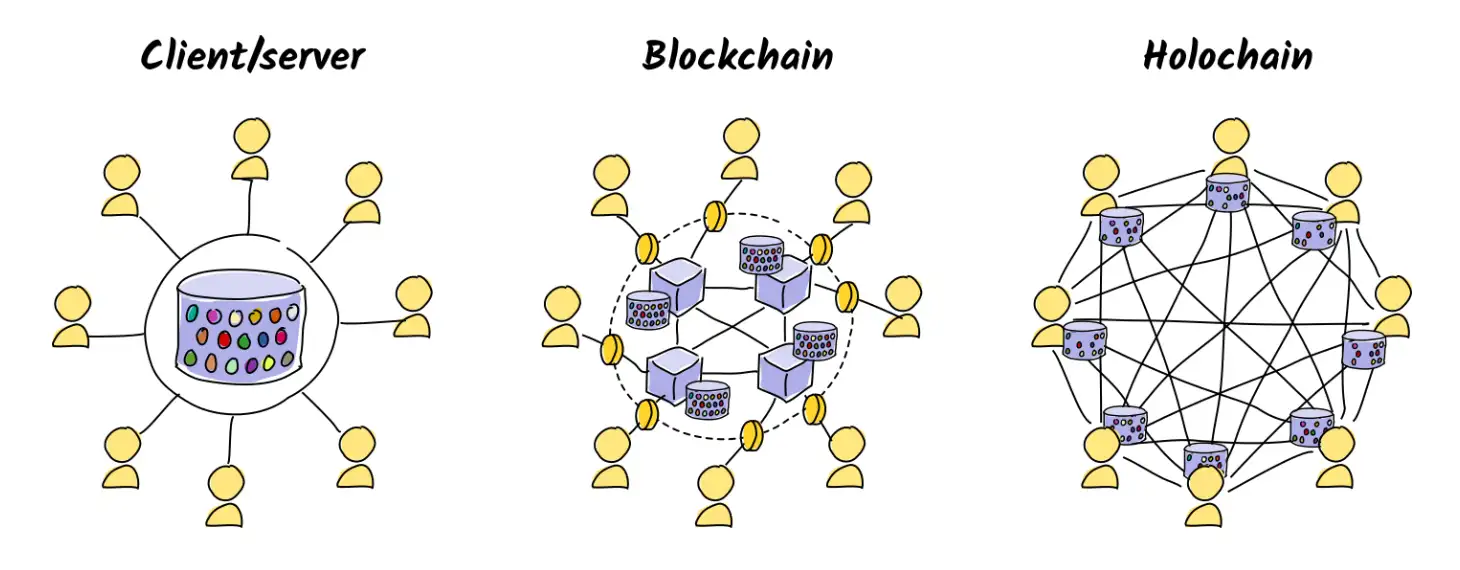
\includegraphics[keepaspectratio]{_i/holochain.png}}

Cette peur paraît infondée, puisque les contrevenants trouvent toujours
des techniques pour échapper à la surveillance. La peur du pire empêche
parfois de s’y préparer. La dictature ne devrait-elle pas être la
crainte première des démocraties? Elles devraient donc s’y préparer, et
nous y préparer. Il est fondamental que des solutions de communication
transversale existent et soient testées, tout comme il était important
que des imprimeries clandestines reproduisent les textes interdits sous
l’occupation nazie.

En 2025, en Occident tout au moins, aucun système répressif ne nous
impose d’échanger nos Livres via des approches Multicast radicales. Par
chance, nous disposons d’autres techniques décentralisées pour nous
protéger de l’influence des algorithmes, qui nous façonnent l’esprit par
touches minuscules, insensibles, imperceptibles, mais répétées jour
après jour, année après année.

L’algorithme a pour but principal de nous rendre addicts à lui-même.
Voilà pourquoi il est si difficile de quitter un réseau social quand on
s’y est installé depuis des années. À partir de 2019, j’ai quasiment
cessé de poster sur Twitter, mais je ne parvenais pas à m’en détacher.
Je n’y ai réussi qu’en\,2023 après la prise de pouvoir de Musk et avant
qu’il ne rebaptise le service X. Les habitudes technologiques se brisent
difficilement, car elles exploitent nos vulnérabilités psychologiques:
notre besoin de connexion sociale, notre désir de récompense immédiate
et notre peur de manquer quelque chose.

En 1948, Aldo Leopold, un des précurseurs de l’écologie,
écrit\footnote{Aldo Leopold, \emph{Almanach d’un comté des sables},
  traduction Éric Chédaille, Gallmeister, 2022.}: «Aucune évolution
importante de l’éthique ne s’est jamais opérée sans un changement
intrinsèque au sein de nos principes intellectuels, de nos loyautés,
affections et convictions.» Une révolution éthique s’impose si nous
voulons résister à la chose. Il est nécessaire de suivre de multiples
cures de désintoxication.

\section{\texorpdfstring{Le retour du
mail}{   }}\label{le-retour-du-mail}

Première méthode: davantage de mails, moins de réseaux sociaux. Notre
adresse mail est le cœur de notre maison numérique. Quand nous
échangeons des messages, aucun algorithme ne décide ce que nous
recevons, excepté les filtres antispam. Pour des données sensibles ou
éviter d’alimenter les IA et les algorithmes de ciblage publicitaire,
nous pouvons crypter les messages ou passer par des services sécurisés
comme Proton Mail\footnote{\href{https://proton.me/fr/mail}{Proton
  Mail}.}.

Sur les plateformes comme Gmail, rien n’empêche les algorithmes de se
nourrir de nos données. Du jour au lendemain, parce que l’administration
Trump l’aurait décidé, Google pourrait fermer notre Gmail. Alors des
sauvegardes régulièrement de nos messages et notre carnet d’adresses
s’imposent. Une bonne solution: utiliser une messagerie libre comme
Thunderbird avec Gmail qui facilite l’archivage\footnote{\href{https://www.thunderbird.net/fr/}{Thunderbird}.}.
En cas de coupure généralisée, rien n’est perdu.

Certains de mes amis activistes remarquent que notre passé numérique
pourra être retourné contre nous, en cas de changement de régime
politique. Ils adoptent un niveau de vigilance maximal, non parce qu’ils
ont quelque chose à cacher aujourd’hui, mais parce que demain des
opinions devenues illicites pourraient leur être reprochées. Mon
intention n’est pas de vous rendre paranoïaque —je ne le suis pas\,—
mais de montrer les risques que la chose nous fait courir.

Quoi qu’il en soit, le mail est l’une des technologies les mieux
immunisées contre la supervision algorithmique. Nos contacts restent nos
contacts. Si nous changeons de boîte mail, nous pouvons les prévenir et
leur communiquer notre nouvelle adresse. Les changements de notre côté
n’impliquent aucun changement du leur, sinon la mise à jour de leur
carnet d’adresses. Comme le courrier postal, le mail nous aide à
construire un réseau social décentralisé, même si nos messages circulent
physiquement sur le réseau Unicast\footnote{Une analogie: un mail doit
  remonter à Paris, voire à New York, avant d’atterrir chez notre
  voisin. Une lettre se contente d’aller à la poste la plus proche et de
  revenir.}.

Quand nous changeons d’adresse postale, nous ne perdons pas nos amis,
c’est une autre affaire sur les réseaux sociaux centralisés. Quand j’ai
quitté Twitter, j’ai abandonné mes milliers de contacts. Je leur ai
envoyé un message pour leur dire que je déménageais, mais la plupart ne
l’ont pas vu et peu ont fait l’effort de me suivre ailleurs. Mon carnet
d’adresses ne m’appartenait pas. Je me suis retrouvé aux prises d’un
système coercitif, comme si on m’avait donné le choix entre rester
prisonnier dans une maison dorée ou être exproprié.

Parce qu’il est notre propriété, notre mail est précieux et nos échanges
par mail aussi. De plus en plus d’éditorialistes quittent les réseaux
sociaux pour créer des newsletters, par exemple avec Substack, Patreon
ou Ghost\footnote{Attention, Substack reste une plateforme centralisée,
  propriétaire, qui récolte des données d’usage des auteurs comme des
  lecteurs, mais il est possible de la quitter en emportant les adresses
  email des abonnés, et de transporter une newsletter sur une autre
  plateforme. Le caractère déménageable des newsletters est très
  important.}. Une newsletter c’est comme un feuilleton distillé
chapitre après chapitre. On se les passe de mail en mail, selon une
logique Multicast.

Ces plateformes de newsletters, parce qu’il s’agit à nouveau de
plateformes, parfois centralisées, bien que technocapitalistes ne sont
pas encore technofascistes. Elles suivront peut-être le même chemin que
beaucoup de GAFAM et finiront par nous imposer les nuisances de leurs
algorithmes. Il est bon de rester vigilant, comme avec toutes les
solutions centralisées qui, quand elles grossissent, gagnent en
puissance et transforment leurs dirigeants en oligarques. Il faut
toujours se préparer à quitter l’adversaire quand on pactise avec lui.
La confiance aveugle est dangereuse. La bonne stratégie: toujours avoir
sa valise prête avec ses données pour émigrer à la moindre alerte.

Le mail reste une des seules façons de nous assurer que nos contacts
reçoivent nos messages. Un mail a une dimension intime, il implique un
lien de confiance entre l’expéditeur et le destinataire, comme entre un
lecteur et son libraire. «Si tu m’adresses ce message, c’est parce que
tu penses qu’il m’intéressera.» Quand on envoie un mail, on peut
décevoir, provoquer la colère, la joie, la tristesse, mais on ne peut
pas se cacher, on accepte implicitement un échange réciproque. C’est
précieux quand, par ailleurs, on essaie tous de parler plus fort que les
autres pour se faire entendre.

Pourquoi peut-on déménager son mail et pas ses comptes sociaux? Pourquoi
ne pouvons-nous pas basculer de Facebook à X, Bluesky, LinkedIn, TikTok
et inversement? Tout simplement parce que ces services sont centralisés,
fermés au monde extérieur, que chacun souhaite nous posséder: nous
sommes des ressources dans le capitalisme de la surveillance. Nous ne
réduirons son emprise qu’en perdant de la valeur à ses yeux.

Outre passer du temps avec les livres, outre utiliser le mail à des fins
sociales et informatives, trois grandes stratégies de résistance sont à
envisager.

\begin{itemize}
\tightlist
\item
  Déposer des bombes.
\item
  Crossposter.
\item
  Rejoindre le Fediverse.
\end{itemize}

\section{\texorpdfstring{Poseur de bombes}{  }}\label{poseur-de-bombes}

Dans les régimes totalitaires, tout opposant devient un terroriste.
Quand nous luttons contre le technofascisme, nous passons du stade
d’adversaire politique à nuisance, surtout si nous militons pour le
Multicast.

Sur un réseau social, quand nous postons un lien vers l’extérieur, ne
serait-ce que la couverture d’un livre, nous incitons nos lecteurs à
voir ailleurs. Poster un lien équivaut à faire exploser une bombe. Trois
règles:

\begin{itemize}
\tightlist
\item
  ne jamais publier d’article en intégralité sur les services
  centralisés (ce qui revient à collaborer avec eux),
\item
  n’y exprimer que rarement des opinions pour ne pas y provoquer des
  débats et y capturer une audience,
\item
  systématiquement renvoyer les lecteurs vers un livre, une newsletter,
  un site personnel, un média indépendant.
\end{itemize}

En dehors des plateformes, copier ses contenus en différents endroits,
voire les distribuer sous forme d’archives lisibles sur n’importe quel
ordinateur en mode Sneakernet. Éviter de s’enfermer en un lieu unique,
donc vulnérable. Oui, c’est compliqué, fatigant, mais c’est la seule
façon d’échapper à la centralisation et à la mainmise des algorithmes.

Dans \emph{L’art de la Guerre}, Sun Tzu écrit: «Hâtez vos préparatifs
lorsque vos adversaires se concentrent; là où ils sont puissants,
évitez-les.» Beaucoup de ses conseils stratégiques pourraient
s’appliquer à la lutte contre la chose: «L’eau, dans son cours, suit la
situation du terrain dans lequel elle coule; de même, votre armée doit
s’adapter au terrain sur lequel elle se meut.» La mobilité, la
dispersion, le désordre apparaissent comme autant de stratégies viables.

En résumé, sur les réseaux centralisés, évitons de nous exprimer
autrement que par des liens vers le monde extérieur, sinon nous
nourrissons la bête de l’intérieur. Chaque contenu offert en pâture
revient à enrichir la chose, peu importent nos opinions. Pour elle,
seule notre présence compte. Nous sommes sa source d’énergie. Mais ne
jamais perdre de vue que nos bombes ont peu d’effet, car peu de nos
contacts les voient et encore moins cliquent dessus.

\section{\texorpdfstring{Crossposteur}{}}\label{crossposteur}

Sun Tzu: «S’il se partage en dix corps [cas des technofascistes chacun
avec sa plateforme], attaquez chacun d’eux séparément avec votre armée
toute entière ; c’est le véritable moyen de combattre toujours avec
avantage. De cette sorte, quelque petite que soit votre armée, le grand
nombre sera toujours de votre côté.» En résumé, publions les mêmes
messages sur différentes plateformes, ce qui s’appelle crossposter, tous
les messages pointant vers la même destination. Les algorithmes
tenteront de nous invisibiliser, mais nous grappillerons de-ci de-là un
peu d’attention.

Face à un adversaire centralisé, jouer la carte de la décentralisation.
Mais attention. Lors de la conquête de l’Ouest, les Apaches, nomades et
mobiles, à la société non hiérarchisée, n’ont jamais été soumis
militairement. On leur a offert des terres pour les sédentariser, puis
des ressources supérieures pour les uns dans le but de hiérarchiser leur
société et de l’asservir.

Tous les réseaux sociaux centralisés adoptent la même stratégie. Ils
concèdent à leurs fidèles davantage de likes, de partages, de visibilité
en échange de la sédentarité. Ils nous notent et nous classent: celui
qui a le plus de vues, de likes, de partages. Ils nous rangent dans des
cases, mettant en avant des quantités plutôt que des qualités,
difficiles à digérer par le capitalisme de la surveillance. Nous sommes
entrés dans une société de la mesure constante. Nous ne sommes plus que
des numéros comme dans la dystopie de Zamiatine.

Pour nous empêcher le crosspost, les réseaux sociaux ont fermé leurs API
(application programming interface), supprimant ainsi la possibilité
pour des services tiers d’automatiser les publications. Quand nous ne
sommes pas geek, nous en sommes réduits à copier-coller nos messages
dans les différents réseaux. Cette tâche fastidieuse est le prix de la
résistance aux injonctions totalitaires. Crossposter revient à jeter du
sable dans les engrenages des algorithmes.

\section{\texorpdfstring{Rejoindre le
Fediverse}{  }}\label{rejoindre-le-fediverse}

Il existe une défense plus radicale. Dès la fin des années\,2000, alors
que les réseaux sociaux centralisés gagnent en puissance, des
développeurs proposent des solutions décentralisées. Le principe:
disposer d’une adresse sociale semblable à une adresse mail. On peut
ainsi discuter avec des correspondants connectés à différents serveurs.
Une «fédération» des «univers», le Fediverse, se forme peu à peu, avec
des plateformes de microblogging similaires à Twitter, la plus populaire
étant Mastodon, mais aussi des services d’échange de photos et de vidéo,
alternatives à Instagram et YouTube\footnote{Sur le Fediverse, voir
  \href{https://fr.wikipedia.org/wiki/Fediverse}{Wikipédia}.}.

Dans la pratique, on ne crée pas un compte Mastodon comme un compte
Facebook, on ouvre un compte sur une instance Mastodon —notre nom sur le
réseau est alors du type @nom@instance, par exemple, on peut me trouver
à l’adresse @tcrouzet@mamot.fr quel que soit le serveur Mastodon auquel
on se connecte. C’est comme avec les mails de type nom@gmail.com ou
nom@orange.fr. Si notre instance nous déplait, parce qu’elle filtrerait
les messages, nous pouvons en changer pour une autre dont la politique
nous satisferait mieux. Dans la pratique, les instances sont non
filtrantes. Le Fediverse ni ne nous enferme ni ne nous supervise. Sa
structure décentralisée empêche toute prise de contrôle. Par ailleurs,
les logiciels qui sous-tendent le Fediverse sont libres et ouverts à
l’analyse et à la critique. Nous pouvons tous lancer de nouvelles
instances.

Le mail appartient au Fediverse depuis toujours. Il existe de nombreux
serveurs mail installables sur n’importe quel ordinateur. Parce que le
mail est décentralisé, aucun technocapitaliste n’a réussi à s’approprier
la technologie. Nous continuons à disposer d’adresses avec des noms de
domaine divers, les boîtes du type @gmail.com ne représentant que 30\,\%
des adresses\footnote{\href{https://www.spocket.co/fr/statistiques/la-dominance-des-clients-de-messagerie}{Très
  exactement 29,7\,\% en 2024}.}. L’idéal est bien sûr de posséder un
mail à son propre nom, ce qui implique d’acheter un nom de domaine.
Ainsi, il est possible de changer de serveur sans prévenir ses contacts.

Pour lutter contre le technofascisme, il est primordial au moins un pied
dans le Fediverse et d’y pratiquer le crossposting des messages publiés
sur les plateformes centralisées, afin que nos lecteurs aient le choix
d’où nous lire, et qu’ils mesurent qu’il n’existe pas un seul internet
mais une myriade de solutions entrecroisées, aussi entremêlées que le
réseau des libraires sur le territoire.

Le Fediverse n’est toutefois pas encore la panacée puisqu’il repose sur
des instances, donc des serveurs sur le réseau Unicast, serveurs de fait
censurables. De nouvelles approches apparaissent qui utilisent les
réseaux Multicast comme Nostr. La résistance s’organise.

\section{\texorpdfstring{Similitudes avec la France de
1940}{     }}\label{similitudes-avec-la-france-de-1940}

Face à la montée de la chose, nous sommes souvent passifs, un peu comme
sous l’occupation quand la plupart des Français poursuivaient leur
train-train. Nombre d’intellectuels qui n’étaient ni collabos ni
pro-nazis ont continué d’écrire dans les titres collabos comme \emph{Le
Matin} ou à publier des livres en toute innocence.

Jocelyn Van Tuyl écrit\footnote{Jocelyn Van Tuyl, \emph{André Gide \& la
  Seconde Guerre mondiale}, Presses universitaires de Lyon, 2017.}:
«Grâce à des révisions soignées et au placement judicieux de ses textes
dans des périodiques associés à la Résistance, Gide crée l’impression
que sa pensée a suivi une trajectoire sans détour, depuis l’inévitable
défaitisme jusqu’à un patriotisme convenable. Cependant, la comparaison
des écrits publiés pendant et après la guerre avec le \emph{Journal} de
Gide révèle l’ambivalence politique persistante de l’auteur.»

Un temps, Gide a publié comme si de rien n’était, alors que beaucoup
d’auteurs basculaient dans la résistance. J’évoque Gide parce qu’il
était le grand écrivain de la période et parce que ça me chagrine de
savoir qu’un auteur que j’ai beaucoup aimé n’a pas toujours été lucide.

Il est inquiétant de constater qu’aujourd’hui la plupart des auteurs,
éditeurs, libraires, bibliothécaires ne prennent pas leur destin en main
et se contentent de communiquer sur les réseaux sociaux centralisés. Ils
oublient que la chose est de facto l’ennemie de la chaîne du livre.

Il est incompréhensible que nos services publics et hommes politiques se
cantonnent aux services centralisés. Ils semblent avoir capitulé face à
la chose, ou pire, ne pas en percevoir l’emprise. Je déplore d’entendre
sur les médias publics citer des sources en provenance des réseaux
centralisés quand elles existent dans le Fediverse (et quand elles
n’existent pas, il faudrait les y pousser). Se cantonner sur les réseaux
centralisés est une forme de défaitisme.

Sur ces réseaux, le plus fort gagne, suivant une logique du «winner
takes all» (le gagnant prend tout et ne laisse que des miettes aux
autres). Cette logique pernicieuse influence les chroniqueurs les mieux
intentionnés, qui finissent par être victimes de la plateforme. Sûrs de
leurs certitudes, ils ne répondent plus aux commentaires et parlent du
haut de leur estrade. Parfois, ils s’indignent de la montée de la chose
à laquelle ils collaborent en attirant plus de monde vers les soleils
dont ils ne sont que des satellites serviles. Les réseaux sociaux
centralisés sont mécaniquement nocifs: ils jouent de notre grégarisme et
fabriquent les oligarques et leurs mignons. Toutes les plateformes
centralisées sont fascisantes.

Heureusement, il subsiste un monde extérieur, au-delà de ce web limité
aux réseaux sociaux centralisés, où la plupart des usagers se lavent
eux-mêmes le cerveau. Il existe encore des sites indépendants, des
blogs, le Fediverse et, en dehors, des livres, des films, des lieux de
rencontre, des espaces où faire société loin du contrôle des
algorithmes.

\section{\texorpdfstring{Partir ou rester?}{  }}\label{partir-ou-rester}

Durant la Seconde Guerre mondiale, des Français ont quitté la France
pour rejoindre les forces libres, d’autres ont rejoint la résistance,
d’autres ont fermé leur gueule, voire collaboré. Nous en sommes au même
point sur internet.

On peut quitter les réseaux sociaux centralisés pour rejoindre les
forces libres décentralisées ou rester connectés aux centres et choisir
la résistance, le silence ou la collaboration. Longtemps, j’ai gardé un
pied du côté des forces libres, un autre du côté de la résistance. Je
restais sur certains réseaux sociaux centralisés pour donner envie
d’aller voir ailleurs, mais tout en écrivant ce texte je me suis dit que
je devais de donner l’exemple.

J’ai quitté Facebook, Instagram, LinkedIn et Bluesky. Les premiers
jours, j’ai éprouvé un effet de manque. Je prenais en main mon téléphone
et ne savais plus quoi en faire faute d’y trouver les applications qui
m’accompagnent depuis des années. C’était douloureux, déstabilisant,
mais peu à peu j’ai découvert un nouvel équilibre: ma récompense, ne
plus subir de contenus toxiques ou de démonstration de narcissisme. J’en
ai vite éprouvé du soulagement. Bonus: j’ai davantage de temps pour
lire.

Des amis auteurs m’ont dit en substance «L’écriture est mon boulot et je
ne peux pas me passer des réseaux sociaux pour le moment, même s’ils
sont problématiques. Ça m’ennuie beaucoup mais sans ça, je peux mettre
la clef sous la porte.» Parfois la droiture intellectuelle implique de
mettre la clé sous la porte. Combien de Français ont continué leur vie
comme si de rien n’était durant l’occupation pour les mêmes raisons?

Migrer vers le Fediverse reste une des manières les plus efficaces de
bousculer les rapports de force et faire pencher la balance du côté de
la démocratie de droit, plutôt que vers la chose en gestation.

Publions hors des réseaux sociaux centralisés, lisons davantage de
livres, inventons de nouvelles fraternités, même si c’est compliqué: une
liberté trop simple n’est souvent qu’une illusion. La liberté a toujours
un coût. Ce n’est pas par hasard si les plateformes centralisées nous
vendent la simplicité à tout prix.

Qui contrôle les réseaux sociaux contrôle le pouvoir. Nous ne défendrons
nos libertés qu’en décentralisant ces monstres, en leur ouvrant le
ventre avec des liens explosifs, voire en prenant nos distances, pour
rechercher à l’extérieur d’autres points de vue, d’autres styles,
d’autres narrations. Si nous censurons Amazon pour acheter ailleurs les
mêmes livres, notre boycott a peu d’utilité. Il est préférable de lutter
contre Amazon en y cherchant les pépites qui s’y cachent. L’important
est d’échapper à la dictature qui nous empêche de penser.

\section{\texorpdfstring{La philosophie du
libre}{   }}\label{la-philosophie-du-libre}

Par principe, les solutions décentralisées sont libres et ouvertes, de
sorte qu’il soit possible d’installer de nouveaux serveurs et d’ouvrir
de nouvelles instances. Un logiciel libre est non privatif. En revanche,
il ne nie ni la paternité de la création ni la possibilité pour le
créateur d’être rémunéré.

Dans \emph{Le Figaro}, Luc Ferry a publié un article inquiétant où il
écrit\footnote{Luc Ferry, ``Le danger mortel de l’open source et des
  deepfakes'', \emph{Le Figaro}, 29 janvier 2025.}: «Mettre les avancées
de l’IA en accès libre laisse l’opportunité aux terroristes, comme au
premier imbécile venu, de détourner le meilleur des projets pour
fabriquer des armes de destruction massive.»

Depuis la première page de ce texte, je m’efforce de montrer que la
centralisation et le secret autour des algorithmes fabriquent la chose,
et Ferry préfère que les IA restent entre quelques mains, qui pourront
en user selon leur bon vouloir. Comment dire? Il y a des technocollabo
qui s’ignorent.

Précision: un logiciel libre est libre d’utilisation, de copie, de
modification et de distribution quand un logiciel open source expose son
code, sans nous donner nécessairement le droit de le modifier ou de le
mettre en œuvre. Un logiciel libre est toujours open source, la
réciproque n’étant pas implicite.

Certes des pirates utilisent parfois des logiciels libres pour mener
leurs attaques. Y aurait-il moins d’attaques s’il y avait moins de
logiciels libres? Non, les crapules développeraient des outils fermés,
plus difficiles à contrer que des outils ouverts. Avec le libre, tout le
monde se bat à armes égales.

Est-ce préférable que tout le monde possède la bombe atomique ou
seulement quelques puissances? J’opte pour la seconde solution, sinon
des dictateurs en fin de règne auraient déjà pressé sur le bouton de
mise à feu. Par analogie, je devrais me ranger à l’avis de Ferry et
juger souhaitable que certains logiciels restent propriétaires et
confidentiels, comme l’arme atomique. Sauf qu’une bombe atomique est
exclusivement une arme, contrairement à un logiciel.

On n’a pas interdit les marteaux parce qu’ils pouvaient dans de rares
cas servir d’armes contondantes. On ne va pas privatiser toutes les IA
au prétexte qu’elles pourraient parfois être mal utilisées. Sinon, il
faudrait interdire beaucoup de choses, les voitures pour commencer,
parfois utilisées pour foncer dans la foule. Avec toutes les
technologies, des risques existent. On ne peut jamais les réduire à
zéro. Fermer les yeux en empêchant tout contrôle sur une technologie est
la pire chose à faire. Mieux vaut ouvrir le capot pour se défendre.

L’ouverture reste dans le cas de l’IA, et de toutes les technologies
potentiellement dangereuses mais non spécifiquement militaires, la moins
pire des solutions. Les réseaux sociaux fabriquent la chose parce que
personne ne contrôle leurs algorithmes faute de transparence. Ces boîtes
noires nous sont imposées unilatéralement. Nous n’avons pas notre mot à
dire, sinon la possibilité de les fuir.

Aux institutions de militer pour l’ouverture. Elles-mêmes devraient
cesser de communiquer sur les réseaux sociaux centralisés et s’appuyer
sur les solutions libres. Si au contraire, elles tentent de centraliser
la société pour mieux la contrôler, elles ne feront que précipiter
l’avènement de la chose.

À l’échelle individuelle, nous pouvons appliquer quelques règles.

\begin{enumerate}
\def\labelenumi{\arabic{enumi}.}
\tightlist
\item
  Limiter nos usages des services centralisés qui n’offrent pas la
  possibilité de les quitter sans perdre le fruit de notre travail
  (c’est malheureusement le cas de la plupart des réseaux sociaux).
\item
  N’utiliser un service que tant qu’il n’est pas néfaste: tous
  commencent par être ouverts avant de se fermer peu à peu et de
  favoriser des thèses souvent contestables (phénomène de
  merdification).
\item
  Se préparer à fuir: à tout moment la situation peut devenir
  éthiquement ou politiquement déplaisante. Par exemple, beaucoup
  d’utilisateurs ont quitté Facebook en 2011 quand le tableau de
  Courbet, \emph{L’Origine du monde}, y a été censuré\footnote{``«L’origine
    du monde»: première victoire d’un David contre le Goliath
    Facebook'',
    \href{https://www.radiofrance.fr/franceculture/podcasts/le-billet-culturel/l-origine-du-monde-premiere-victoire-d-un-david-contre-le-goliath-facebook-9749421}{\emph{France
    Culture}}, 2 février\,2018.}.
\item
  Avoir plus qu’un pied dans le Fediverse: y être actif, sinon c’est
  être défaitiste.
\item
  Bien sûr, lire des Livres loin de l’agitation du temps réel et des
  algorithmes.
\item
  Garder espoir. Quand Musk s’est mit à délirer, les ventes de Tesla se
  sont effondrées, peuvent que nous autres utilisateurs/consommateurs ne
  sommes pas impuissants\footnote{``Tesla’s Earnings Are Even More
    Brutal Than We Expected'',
    \href{https://futurism.com/tesla-earnings-brutal-elon-musk}{Futurism},
    22 avril 2025.}.
\end{enumerate}

\chapter{\texorpdfstring{Lire, c’est
résister}{  }}\label{lire-cest-ruxe9sister}

Quand le fascisme s’installe, il commence par contrôler l’information.
La chose ne fait pas exception, mais elle agit au nom de la liberté
d’expression. Nous croyons choisir alors que des algorithmes nous
choisissent. Nous pensons nous exprimer alors que nous alimentons des
machines à avaler nos données.

Face à cette menace, le Livre est notre meilleure défense. Il échappe à
l’emprise des oligarques. Chaque Livre est un acte de résistance, chaque
librairie un bastion de liberté, chaque lecteur un combattant potentiel.

Il ne s’agit pas de rejeter la technologie, mais de préserver des
espaces loin de la supervision des monstres centralisés. Les Livres nous
offrent de précieuses parenthèses où notre imagination peut vagabonder,
s’épanouir sans surveillance, mûrir loin des injonctions marchandes.

Les signes avant-coureurs de la chose sont là, de plus en plus visibles.
Réveillons-nous avant que son emprise ne se généralise. Chaque heure
passée à lire, chaque discussion autour d’un texte plutôt que sur un
réseau social centralisé est une victoire.

Les Livres sont nos alliés dans cette guerre asymétrique contre les
technocollabos. À nous de les faire circuler, de les partager, de les
défendre. À nous de préserver ce réseau décentralisé de librairies et de
bibliothèques qui maille nos territoires. À nous de résister, page après
page, mot après mot.

À travers les Livres, nous défendons notre liberté de penser, notre
droit à la pluralité, notre capacité à imaginer d’autres futurs. Le
Livre contre-attaque. Rejoignez le combat: lisez davantage, scrollez
moins!

% Afficher les notes à la fin du document
\clearpage
\begingroup
\parindent 0pt
\parskip 1ex
\def\enotesize{\small}
\theendnotes
\endgroup



\end{document}